\documentclass[11pt,a4paper]{article}

\usepackage[margin=1in]{geometry}
\usepackage[T1]{fontenc}
\usepackage[utf8]{inputenc}
\usepackage{mathptmx}
\usepackage{amsmath,amssymb,amsfonts,amsthm}
\usepackage{mathtools}
\usepackage{graphicx}
\usepackage{booktabs}
\usepackage{multirow}
\usepackage{array}
\usepackage{xcolor}
\usepackage{microtype}
\usepackage{url}
\usepackage{cite}
\usepackage{authblk}
\def\UrlBreaks{\do\/\do-\do\_\do.}
\renewcommand{\_}{\textunderscore\allowbreak}
\emergencystretch=1.5em
\usepackage[colorlinks=true,linkcolor=blue!60!black,citecolor=blue!60!black,urlcolor=blue!60!black]{hyperref}
\pdfstringdefDisableCommands{%
  \def\SM{SonarMoE}%
  \def\OD{OblivDispatch}%
}

\graphicspath{{figures/}}

\newtheorem{theorem}{Theorem}
\newtheorem{lemma}{Lemma}
\newtheorem{proposition}{Proposition}
\newtheorem{corollary}{Corollary}
\theoremstyle{definition}
\newtheorem{definition}{Definition}
\theoremstyle{remark}
\newtheorem{remark}{Remark}

\newcommand{\SM}{\textsc{SonarMoE}}
\newcommand{\OD}{\textsc{OblivDispatch}}
\newcommand{\MLB}{\textsc{MoELeak-Bench}}

\title{\Large\bfseries SonarMoE: Remote Prompt and Tool-Schema Reconstruction via Expert Contention in Disaggregated MoE Serving and Differentially Private Mitigation}

\author[1,*]{Mohammed Kamran Syed}
\author[2]{Anudeep Rentala}
\author[2]{Somesh Rahul}
\author[3]{Raghuram Malpe Pai}
\author[3]{Krishna Suman Dara}

\affil[1]{Independent Researcher, Mountain House, CA, USA \newline\small\texttt{mohammedkamran.syed@ieee.org} (Corresponding Author; ORCID: 0009-0009-9058-5375)}
\affil[2]{Independent Researcher, Fremont, CA, USA \newline\small\texttt{anudeep.rentala@ieee.org}, \texttt{someshrahul@ieee.org}}
\affil[3]{Independent Researcher, Sunnyvale, CA, USA \newline\small\texttt{raghuram.pai@ieee.org}, \texttt{krishna-suman.dara@ieee.org}}

\date{}

\begin{document}

\maketitle

\begin{abstract}
Large Mixture-of-Experts (MoE) serving systems often split Attention from feed-forward computation, a design known as Attention--FFN Disaggregation (AFD). Each tenant gets its own Attention server and Key-Value (KV) cache, while all tenants share a common pool of Expert-Parallel GPUs. Because tenants do not share KV caches or physical hosts, operators usually treat AFD as safe from cross-tenant inference leaks. We show that this assumption fails. An outside user with only a normal HTTP streaming API key can still infer a co-scheduled victim's prompt domain and Model Context Protocol (MCP) tool calls from shared expert contention. Our attack, \SM{}, finds rank-concentrated canary tokens offline from public router weights without seeing any victim data, and sizes each canary batch right below a GPU matrix-multiply tile boundary ($N_{\mathrm{can}} = M_{\mathrm{tile}} - 6 = 122$). When a victim sends even a few tokens to a primed expert, the batch crosses the tile boundary and adds a discrete microsecond delay to the attacker's streamed response. Using Apple M5 Pro FP16 kernel profiling, hardware-grounded AFD simulation with synthetic jitter, and live localhost HTTP/1.1 SSE tests on \texttt{OLMoE-1B-7B} and \texttt{Granite-3.1-MoE} under strict constant-length windows ($B_{\mathrm{vic}} = 64$, $0.00$~bits of length leakage), \SM{} reaches $87.0\%$ five-domain accuracy and $90.0\%$ Top-1 accuracy across $20$ MCP tool schemas. To stop this leak, we build \OD{}, a per-tenant defense that redirects hot-expert overflow into idle barrier slack and adds shifted two-sided Gaussian padding with data-independent clipping. \OD{} drops attacker accuracy to random guessing while using $2.4\times$ FFN compute (versus $8.0\times$ for uniform padding) and adding only $+0.15$ perplexity (versus $+13.9$ to $+630.3$ for pure router noise).

\medskip
\noindent\textbf{Keywords:} Mixture-of-Experts; Disaggregated LLM serving; GPU tile quantization; Remote timing side channels; Model Context Protocol; Differential privacy; Straggler-slack scheduling.
\end{abstract}

% ============================================================================
\section{Introduction}\label{sec:intro}
% ============================================================================

Sparse Mixture-of-Experts (MoE) language models grow capacity without raising per-token compute by routing each token to only a small top-$k$ subset of feed-forward networks (FFNs)~\cite{shazeer2017outrageously,fedus2022switch}. Open-weight models such as \texttt{DeepSeek-V2/V3/R1}~\cite{deepseek2024v2,deepseek2025v3,deepseek2025r1}, \texttt{Qwen2-MoE}~\cite{yang2024qwen2moe}, \texttt{Mixtral}~\cite{jiang2024mixtral}, and \texttt{OLMoE}~\cite{muennighoff2025olmoe} pick $2$ to $8$ experts out of $32$ to $256$ at every layer. Over training, individual experts become strongly tied to specific topics such as clinical notes, SQL queries, payment APIs, cryptographic code, or legal contracts~\cite{dai2024deepseekmoe}.

Running these large MoE models cheaply in the cloud creates a well-known memory bottleneck: expert weights need large batches to stay busy, while Attention Key-Value (KV) caches grow rapidly with batch size~\cite{kwon2023vllm,zheng2024sglang,zhong2024distserve,patel2024splitwise}. Modern serving systems solve this with \emph{Attention--FFN Disaggregation (AFD)}, used in \texttt{MegaScale-Infer}~\cite{zhu2025megascaleinfer} and \texttt{DeepEP}~\cite{zhao2025deepep}. Under AFD, Victim~A (for example, a hospital assistant or payment agent) runs self-attention on Dedicated Attention Server~1 with a private KV cache, while Attacker~B (an ordinary external API customer) runs self-attention on Attention Server~2. At every MoE layer, however, both servers send their post-attention vectors into the \emph{same shared pool of Expert-Parallel (EP) GPUs} so the cluster can amortize expert memory across tenants.

Cloud operators often assume AFD blocks cross-tenant side channels because prior LLM attacks rely on shared state that AFD removes. Cache-probing attacks such as \texttt{PROMPTPEEK}~\cite{wu2025promptpeek} and \texttt{InputSnatch}~\cite{zheng2025inputsnatch} need shared KV or semantic caches and leak zero bits when Attention servers are isolated. Local microarchitectural attacks such as \texttt{MoEcho}~\cite{ding2025moecho} need code execution on the victim's physical host to read CPU/GPU TLBs or hardware counters. Network attacks such as \texttt{Whisper Leak}~\cite{microsoft2025whisperleak} need a wiretap on the victim's own network path, and white-box routing attacks~\cite{patel2026routingmembership} assume the API returns raw gate logs.

We show that remote HTTP streaming timestamps alone still leak what a victim is asking whenever disaggregated Attention servers share an Expert pool. On each Expert Rank $p \in \{1, \dots, P\}$, GPU matrix-multiply (\texttt{GEMM}) kernels split the token batch into fixed hardware tiles~\cite{gale2023megablocks,tan2025gpugemmcliff}. As a result, execution time behaves like a staircase rather than a smooth line. On an Apple M5 Pro GPU running \texttt{OLMoE-1B-7B} $\mathrm{FP16}$ experts, moving from $N=64$ to $N=65$ tokens adds just $+3.43~\mu\mathrm{s}$, whereas crossing the tile boundary from $N=128$ to $N=129$ jumps by $+27.71~\mu\mathrm{s}$ per expert ($+443~\mu\mathrm{s}$ across $16$ layers). Standard sparse MoE runtimes also skip launching experts that receive zero tokens ($0~\mu\mathrm{s}$ versus $72$--$90~\mu\mathrm{s}$), creating a second sharp step.

Our attack, \SM{}, turns these hardware steps into a remote timing oracle. Offline, without seeing any victim prompts, \SM{} screens the model's public vocabulary to find a small set of single-token \emph{Canary Probes} that concentrate onto chosen Expert Ranks. Attacker~B repeats a canary token $N_{\mathrm{can}} = M_{\mathrm{tile}} - \delta$ times (such as $122$ tokens for $M_{\mathrm{tile}} = 128$, $\delta = 6$) on Attention Server~2. This parks the target experts right below the $128$-token cliff and forces the cross-rank barrier onto Target Rank $p^*$. Whenever Victim~A's co-scheduled prefill chunk sends more than $\delta$ tokens to those same experts, the combined batch spills into the next GPU tile and leaves a clear Inter-Token Latency ($\mathrm{ITL}$) echo in Attacker~B's HTTP stream.

Stopping this leak cheaply is hard. Padding every expert to the worst-case batch size multiplies FFN work by $4\times$ to $8\times$, while adding heavy noise to the router destroys language quality. We design \OD{}, a per-tenant $(\epsilon, \delta)$-differentially private dispatcher built on \emph{Straggler-Slack Hiding}. In normal $\text{top-}k$ MoE serving, every layer waits for its slowest (most loaded) rank at the combine barrier, leaving lighter ranks idle for $180$--$320~\mu\mathrm{s}$. Before tenants are batched together, \OD{} caps Victim~A's hot experts by spilling excess tokens into Victim~A's own lightest local slots, runs at least $N_{\min} = 1$ token per expert to close the zero-token skip channel, and blinds per-expert counts with shifted two-sided Gaussian noise and data-independent clipping $[N_{\min}, N_{\max}]$.

We test \SM{} and \OD{} on two open-weight MoE models: \texttt{allenai/\allowbreak OLMoE-1B-7B-\allowbreak 0924-Instruct} (unnormalized $\text{top-}8$ routing, $64$ experts, $16$ layers) and \texttt{ibm-granite/\allowbreak granite-3.1-1b-\allowbreak a400m-instruct} (normalized $\text{top-}8$ routing, $32$ experts, $24$ layers). Our evaluation combines real Apple M5 Pro $\mathrm{FP16}$ kernel profiling, hardware-grounded AFD simulation across synthetic jitter $\sigma_{\mathrm{net}} \in \{10, 50, 200\}~\mu\mathrm{s}$, and a live \texttt{127.0.0.1} HTTP/1.1 Server-Sent Events (SSE) loopback server. Every query in our two-tier \MLB{} benchmark ($100$ prompts across $5$ domains and $160$ JSON-RPC prefill chunks across $20$ Model Context Protocol~\cite{anthropic2024mcp,patil2024bfcl} tool schemas) is fixed to exactly $B_{\mathrm{vic}} = 64$ tokens so prompt length leaks $0.00~\mathrm{bits}$.

This paper makes four main contributions:
\begin{enumerate}
  \item \textbf{Tile-Boundary Channel Theory:} We model remote timing leakage across shared Expert pools and prove \emph{Theorem~\ref{thm:capacity}}, showing that tile-boundary canary sizing ($N_{\mathrm{can}} = M_{\mathrm{tile}} - \delta$) boosts single-probe channel capacity by $2.9\times$ to $17.8\times$ over uncalibrated probes under network jitter ($\sigma_{\mathrm{net}} \in [50, 200]~\mu\mathrm{s}$).
  \item \textbf{Blind Canary Probing and Deconvolution (\SM{}):} We build an offline vocabulary profiler and common-mode-rejected decoder that need no victim data during setup. Under zero length leakage on \texttt{OLMoE-1B-7B}, \SM{} reaches $87.0 \pm 7.6\%$ blind $5$-domain accuracy ($\sigma_{\mathrm{net}} = 50~\mu\mathrm{s}$) and $90.0 \pm 3.5\%$ Top-1 ($94.4 \pm 1.3\%$ Top-3) accuracy across $20$ MCP tool schemas ($\sigma_{\mathrm{net}} = 10~\mu\mathrm{s}$; $87.5\%$ Top-1 versus $40.6\%$ for naive $N=16$ probes at $\sigma_{\mathrm{net}} = 50~\mu\mathrm{s}$).
  \item \textbf{Per-Tenant \OD{}, Baselines, and Ablations:} We prove \emph{Theorem~\ref{thm:dp_bound}}, showing that shifted two-sided Gaussian count blinding with data-independent clipping and split failure accounting ($\delta = \delta_{\mathrm{zCDP}} + \delta_{\mathrm{tail}}$) guarantees query-level $(\epsilon, \delta)$-DP. Across $3$ seeds and full defense baselines, \OD{} drops $5$-domain accuracy to the $20.0\%$ random floor ($0$ underflow slots) and $20$-way MCP accuracy to $1.3\%$--$6.3\%$ ($\le 0.065~\mathrm{bits}$ MI) at $2.40\times$ FFN compute (versus $8.00\times$ for uniform padding) and $+0.08$ to $+0.15$ perplexity shift on an expanded $24$-passage corpus (versus $+13.9$ to $+630.3$ for pure router noise).
  \item \textbf{Open Benchmark and Live SSE Verification:} We release \MLB{} ($260$ constant-length queries plus our $24$-passage perplexity corpus) and test \SM{} and \OD{} end-to-end over $12{,}928$ live loopback TCP/HTTP-1.1 SSE frames executing real MPS GPU kernels.
\end{enumerate}


\begin{figure}[htbp]
  \centering
  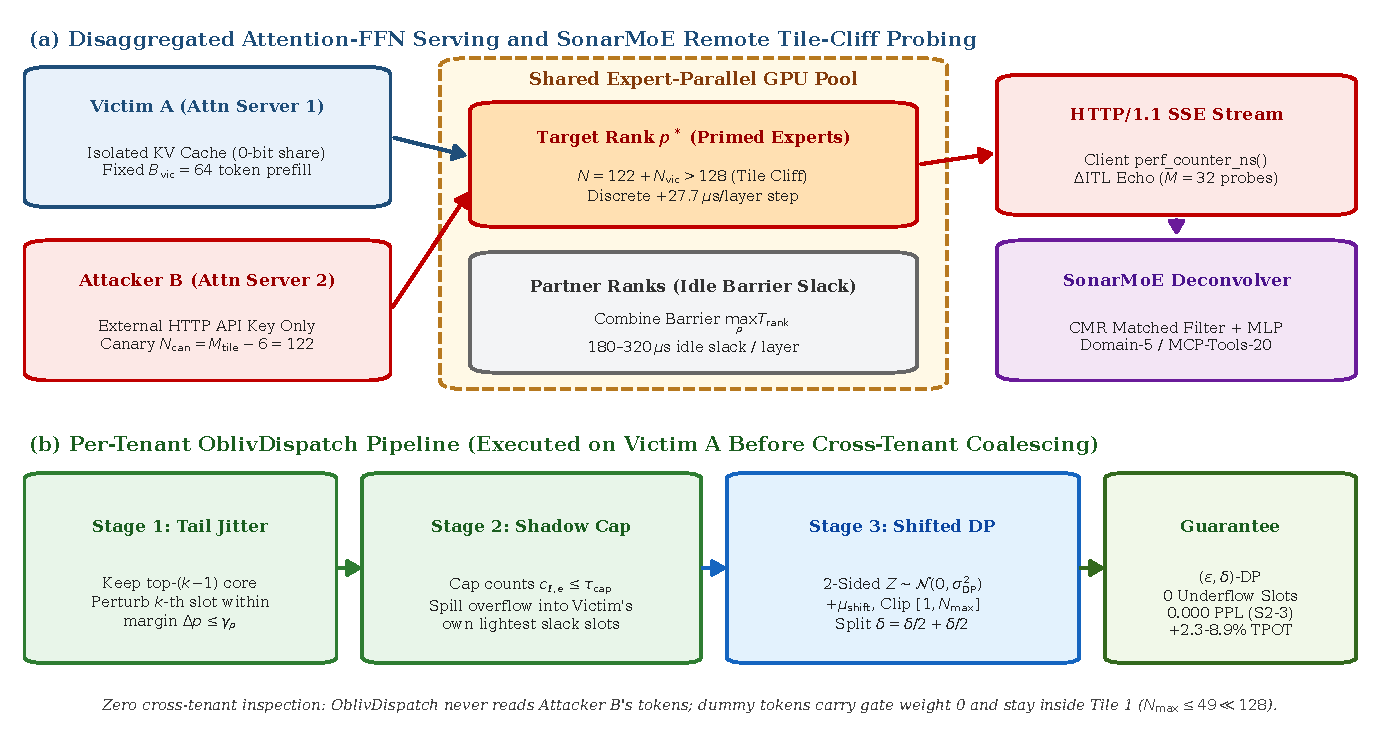
\includegraphics[width=0.98\textwidth]{fig0_system_architecture.pdf}
  \caption{System architecture and mitigation overview. (a) Disaggregated Attention--FFN serving isolates tenant KV caches across separate Attention servers, yet co-scheduled tokens share Expert-Parallel GPU ranks where tile-primed canaries ($N_{\mathrm{can}} = M_{\mathrm{tile}} - 6 = 122$) convert victim routing into discrete $+27.7~\mu\mathrm{s}$/layer HTTP/SSE latency echoes. (b) Per-tenant three-stage \OD{} caps hot-expert counts into Victim~A's own idle combine-barrier slack and applies shifted two-sided Gaussian count blinding with data-independent clipping $[1, N_{\max}]$ before cross-tenant coalescing.}
  \label{fig:arch}
\end{figure}

Figure~\ref{fig:arch} summarizes the disaggregated contention channel and our per-tenant mitigation pipeline. The remainder of this paper is organized as follows. Section~\ref{sec:background} reviews sparse MoE routing and AFD combine barriers. Section~\ref{sec:threat} defines our remote threat model. Section~\ref{sec:attack} develops \SM{} and proves Theorem~\ref{thm:capacity}. Section~\ref{sec:defense} presents \OD{} and proves Theorem~\ref{thm:dp_bound}. Sections~\ref{sec:methodology} and~\ref{sec:eval} describe \MLB{} and our hardware evaluation, followed by related work in Section~\ref{sec:related}, limitations in Section~\ref{sec:discussion}, and conclusions in Section~\ref{sec:conclusion}.

% ============================================================================
\section{Background and Disaggregated MoE Serving}\label{sec:background}
% ============================================================================

\subsection{Sparse Top-$k$ Routing Semantics}
Consider an $L$-layer MoE transformer with hidden dimension $H$, vocabulary $\mathcal{V}$, and $E$ routed experts per layer. Given post-attention normalized hidden state $h_{\ell, u} \in \mathbb{R}^H$ for token $u$ at layer $\ell \in \{0, \dots, L-1\}$, the router computes gate logits $z_{\ell, u} = W_{\mathrm{gate}}^{(\ell)} h_{\ell, u} \in \mathbb{R}^E$. Modern open-weight MoE families instantiate two top-$k$ normalization conventions:
\begin{enumerate}
  \item \emph{Full-Vocabulary Softmax Routing (\texttt{OLMoE}, \texttt{Qwen-MoE}):} Probabilities $p_{\ell, u} = \mathrm{softmax}(z_{\ell, u})$ are computed over all $E$ experts first, and the router selects index set $\mathcal{S}_{\ell, u} = \mathrm{TopK}(p_{\ell, u}, k)$ without renormalizing ($\sum_{e \in \mathcal{S}_{\ell, u}} p_{\ell, u, e} < 1$)~\cite{muennighoff2025olmoe,yang2024qwen2moe}.
  \item \emph{Top-$k$ Renormalized Routing (\texttt{Mixtral}, \texttt{Granite-MoE}):} The router selects $\mathcal{S}_{\ell, u} = \mathrm{TopK}(z_{\ell, u}, k)$ and normalizes weights strictly across the active subset via $w_{\ell, u, e} = \exp(z_{\ell, u, e}) / \sum_{j \in \mathcal{S}_{\ell, u}} \exp(z_{\ell, u, j})$~\cite{jiang2024mixtral,gale2023megablocks}.
\end{enumerate}
Each selected expert $e \in \mathcal{S}_{\ell, u}$ evaluates a gated SwiGLU MLP:
\begin{equation}\label{eq:swiglu}
  f_{\ell, e}(h) = W_{\mathrm{down}}^{(\ell, e)} \Big( \mathrm{SiLU}\!\big(W_{\mathrm{gate}}^{(\ell, e)} h\big) \odot \big(W_{\mathrm{up}}^{(\ell, e)} h\big) \Big),
\end{equation}
and the layer output accumulates $\sum_{e \in \mathcal{S}_{\ell, u}} w_{\ell, u, e} f_{\ell, e}(h_{\ell, u})$ using the SwiGLU operator in~\eqref{eq:swiglu}.

\subsection{Attention--FFN Disaggregation (AFD)}
In conventional colocated serving, replicating $E = 64$--$256$ expert MLPs across small decode batches leaves expert HBM bandwidth severely underutilized, while large batches exhaust KV-cache capacity~\cite{zhu2025megascaleinfer}. AFD resolves this tension by splitting inference into two pools connected via RoCEv2 or InfiniBand RDMA (\texttt{DeepEP}~\cite{zhao2025deepep}):
\begin{itemize}
  \item \emph{Isolated Attention Frontends:} Tenant requests are pinned to separate Attention replicas. Each replica maintains tenant-local paged KV caches~\cite{kwon2023vllm}, computes causal self-attention and router top-$k$ indices $\mathcal{S}_{\ell, u}$, and transmits tuples $(h_{\ell, u}, \mathcal{S}_{\ell, u})$ to the Expert Pool.
  \item \emph{Shared Expert-Parallel Backend:} The $E$ experts at layer $\ell$ are partitioned across $P$ Expert Ranks, where Rank $p \in \{0, \dots, P-1\}$ hosts local subset $\mathcal{E}_p$ of size $E_{\mathrm{loc}} = E / P$. During micro-batch tick $t$, Rank $p$ coalesces incoming hidden vectors from all co-scheduled Attention frontends destined for each $e \in \mathcal{E}_p$, executes the corresponding expert \texttt{GEMM}s, and returns output vectors via an RDMA \texttt{combine} operation.
\end{itemize}

Two combine synchronization modes appear in deployed AFD engines. Under a \emph{Global Synchronous Barrier} (standard collective all-to-all combine), all Attention frontends participating in tick $t$ wait for the slowest Expert Rank across the entire pool, incurring layer delay $\max_{p \in \{0, \dots, P-1\}} T_{\mathrm{rank}}(\ell, p)$. Under \emph{Selective Asynchronous Combine} (\texttt{DeepEP} low-latency GPUDirect RDMA / IBGDA~\cite{zhao2025deepep}), an Attention frontend waiting on a specific request completes as soon as the subset of ranks $\mathcal{P}_{\ell} \subseteq \{0, \dots, P-1\}$ referenced by its dispatched tokens returns completions, incurring $\max_{p \in \mathcal{P}_{\ell}} T_{\mathrm{rank}}(\ell, p)$. We analyze and evaluate both modes, treating the stricter Global Synchronous Barrier as our primary conservative baseline.

\subsection{GPU Tile Quantization and Zero-Token Kernel Skipping}
Let $N_{\ell, e}(t) = N_{\ell, e}^{\mathrm{vic}}(t) + N_{\ell, e}^{\mathrm{can}}(t)$ denote the total co-batched tokens routed to expert $e \in \mathcal{E}_p$ in tick $t$. Sparse MoE runtimes exhibit two discrete hardware nonlinearities:
\begin{enumerate}
  \item \emph{Zero-Token Kernel Skipping:} As implemented in standard PyTorch/Transformers, \texttt{vLLM}, and \texttt{SGLang} dispatchers (\texttt{expert\_hit = nonzero(counts > 0)}), if $N_{\ell, e}(t) = 0$, the runtime issues zero GPU kernel launches for expert $e$. Moving from $N_{\ell, e} = 0$ to $N_{\ell, e} = 1$ incurs fixed kernel launch and weight-fetch latency $\tau_{\mathrm{launch}} > 0$ ($78$--$95~\mu\mathrm{s}$ on M5 Pro $\mathrm{FP16}$ for \texttt{OLMoE}).
  \item \emph{Hardware Tile-Boundary Stepping:} For $N_{\ell, e}(t) \ge 1$, GPU matrix-multiply kernels partition the token dimension $M = N_{\ell, e}(t)$ into fixed hardware threadgroup tiles of height $M_{\mathrm{tile}}$ (typically $64$ or $128$)~\cite{tan2025gpugemmcliff}. Within a single tile ($1 \le N_{\ell, e} \le M_{\mathrm{tile}}$), weight matrices $W_{\mathrm{gate/up}}^{(\ell, e)}$ and $W_{\mathrm{down}}^{(\ell, e)}$ are streamed from HBM/SLC once and arithmetic lanes are amortized in parallel, producing a nearly flat slope $\alpha_{\mathrm{in}} \ll 1~\mu\mathrm{s}/\text{token}$. Crossing $N_{\ell, e} = m M_{\mathrm{tile}} + 1$ forces a second wave of weight-tile reads and threadgroup dispatches, adding discrete step $\Delta_{\mathrm{tile}} \gg \alpha_{\mathrm{in}}$:
\end{enumerate}
\begin{equation}\label{eq:piecewise_latency}
  T_{\mathrm{exp}}(N) = \mathbb{I}[N > 0] \left( \tau_{\mathrm{base}} + \alpha_{\mathrm{in}} N + \Delta_{\mathrm{tile}} \left\lfloor \frac{N - 1}{M_{\mathrm{tile}}} \right\rfloor \right) + \xi_{\mathrm{gpu}},
\end{equation}
where $\xi_{\mathrm{gpu}}$ denotes sub-microsecond hardware execution jitter.

\begin{table}[htbp]
  \centering
  \caption{Comparison of \SM{} Against Closest 2024--2026 LLM Side-Channel and MoE Security Prior Art.}
  \label{tab:prior_art}
  \renewcommand{\arraystretch}{1.12}
  \resizebox{\textwidth}{!}{%
  \begin{tabular}{lcccccc}
    \toprule
    \textbf{Attack / Study} & \textbf{Security Goal} & \textbf{Zero Host / Counter Access} & \textbf{Zero Shared KV / Prefix Cache} & \textbf{Zero Victim Link Sniffing} & \textbf{Black-Box HTTP API Only} & \textbf{Formal DP Defense Included} \\
    \midrule
    \texttt{PROMPTPEEK} (NDSS'25)~\cite{wu2025promptpeek} & Confidentiality & \checkmark & $\times$ (Needs shared KV) & \checkmark & \checkmark & $\times$ \\
    \texttt{InputSnatch} (USENIX'25)~\cite{zheng2025inputsnatch} & Confidentiality & \checkmark & $\times$ (Needs semantic cache) & \checkmark & \checkmark & $\times$ \\
    \texttt{Whisper Leak} (2025)~\cite{microsoft2025whisperleak} & Confidentiality & \checkmark & \checkmark & $\times$ (Needs TLS MITM) & $\times$ & $\times$ \\
    \texttt{MoEcho} (ACM CCS'25)~\cite{ding2025moecho} & Confidentiality & $\times$ (Local CPU/GPU TLB) & \checkmark & \checkmark & $\times$ & $\times$ \\
    Routing Membership (PoPETs'26)~\cite{patel2026routingmembership} & Confidentiality & \checkmark & \checkmark & \checkmark & $\times$ (Needs gate logs) & $\times$ \\
    Trigger the Straggler (2026)~\cite{liu2026straggler} & Availability (DoS) & \checkmark & \checkmark & \checkmark & \checkmark & $\times$ \\
    \midrule
    \textbf{\SM{} + \OD{} (Ours)} & \textbf{Confidentiality + DP} & \textbf{\checkmark} & \textbf{\checkmark} & \textbf{\checkmark} & \textbf{\checkmark} & \textbf{\checkmark\ ($(\epsilon,\delta)$-DP)} \\
    \bottomrule
  \end{tabular}%
  }
\end{table}

% ============================================================================
\section{Threat Model and Prior-Art Differentiation}\label{sec:threat}
% ============================================================================

\emph{System Model:} A cloud provider operates a multi-tenant AFD cluster serving a known open-weight MoE model (such as \texttt{OLMoE}, \texttt{DeepSeek-V2/V3}, \texttt{Qwen-MoE}, or \texttt{Granite-MoE}). Cross-tenant KV-cache sharing and semantic prompt caching are strictly disabled. Victim~A and Attacker~B are scheduled onto physically separate Attention frontend instances (Attention Server~1 and Attention Server~2) that dispatch hidden states to a shared $P$-rank Expert GPU pool.

\emph{Adversary Capabilities:} Attacker~B is an unprivileged external customer holding a standard commercial HTTP/HTTPS streaming API key (\texttt{text/event-stream} SSE). Attacker~B has \emph{zero} code-execution, container, OS, CPU cache, GPU TLB, or performance-counter access on any cluster node; \emph{zero} access to Victim~A's network link or TLS ciphertexts; and \emph{zero} access to router logits or expert load telemetry in API responses. Attacker~B can submit ordinary token sequences to Attention Server~2 and record client-side arrival timestamps $t_0, t_1, \dots, t_R$ of streamed response chunks at microsecond resolution using standard monotonic clocks (\texttt{clock\_gettime} / \texttt{perf\_counter\_ns}), yielding observed Inter-Token Latencies $\mathrm{ITL}_r = t_r - t_{r-1}$ corrupted by additive network and OS scheduling jitter $\eta_r \sim \mathcal{N}(0, \sigma_{\mathrm{net}}^2)$.

\emph{Adversary Goal:} While Victim~A processes a confidential enterprise prompt or invokes an internal Model Context Protocol (MCP) tool schema (such as \texttt{stripe\_issue\_refund}, \texttt{fhir\_patient\_medication\_order}, or \texttt{kms\_aes\_gcm\_envelope\_seal}), Attacker~B aims to infer Victim~A's semantic domain or exact invoked MCP tool class $Y \in \{1, \dots, K\}$ purely from streamed canary $\Delta\mathrm{ITL}$ observations, even when all victim requests have identical token length $B_{\mathrm{vic}}$ so total cluster load carries zero class information. Table~\ref{tab:prior_art} summarizes how this threat model strictly separates \SM{} from all five closest $2025$--$2026$ studies~\cite{wu2025promptpeek,zheng2025inputsnatch,microsoft2025whisperleak,ding2025moecho,patel2026routingmembership,liu2026straggler}.

% ============================================================================
\section{SonarMoE Remote Contention Attack}\label{sec:attack}
% ============================================================================

\begin{figure}[htbp]
  \centering
  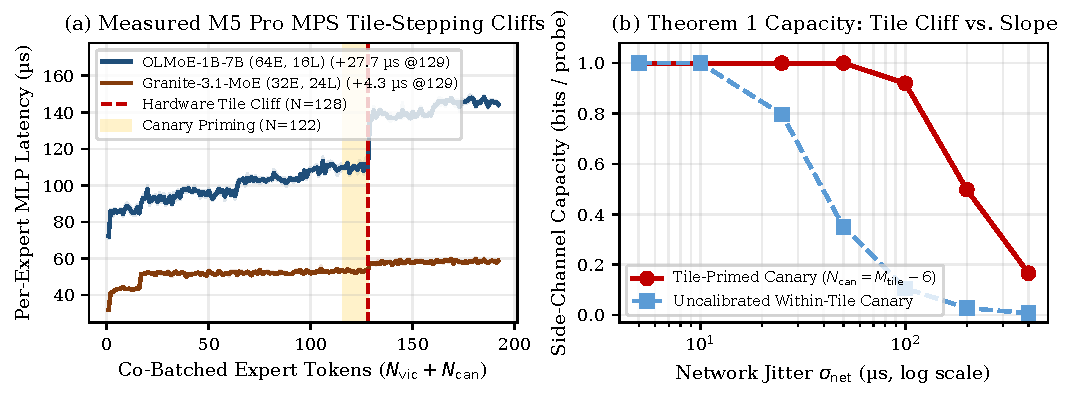
\includegraphics[width=0.94\textwidth]{fig1_tile_cliff_capacity.pdf}
  \caption{Empirical hardware tile quantization and analytical side-channel capacity. (a) Measured Apple M5 Pro MPS $\mathrm{FP16}$ per-expert MLP latency across co-batched token counts $N \in [1, 192]$ on real \texttt{OLMoE-1B-7B} and \texttt{Granite-3.1-MoE} weights, revealing a sharp hardware tile step at $N = 128 \to 129$ right above the $N_{\mathrm{can}} = 122$ priming zone. (b) Exact per-probe side-channel capacity under Theorem~\ref{thm:capacity} across network jitter $\sigma_{\mathrm{net}} \in [5, 400]~\mu\mathrm{s}$ ($R=6$ streamed tokens).}
  \label{fig:tile_cliff}
\end{figure}

\subsection{Tile-Boundary Channel Amplification Theory}
Suppose Attacker~B streams $R$ tokens for Canary Probe $c_m$ while Victim~A dispatches a $B_{\mathrm{vic}}$-token chunk. On Expert Rank $p$, execution latency at layer $\ell$ sums over local experts:
\begin{equation}\label{eq:rank_lat}
  T_{\mathrm{rank}}(\ell, p) = \sum_{e \in \mathcal{E}_p} T_{\mathrm{exp}}\!\left(N_{\ell, e}^{\mathrm{vic}} + N_{\ell, e}^{\mathrm{can}}(c_m)\right).
\end{equation}
Under a global synchronous combine barrier over~\eqref{eq:rank_lat}, two obstacles confront a naive attacker who sends a short canary sequence ($N_{\mathrm{can}} \ll M_{\mathrm{tile}}$). First, if Victim~A's prompt creates a hot straggler on some rank $q \neq p^*$, then $\max_p T_{\mathrm{rank}}(\ell, p)$ locks onto Rank~$q$ across every probe $m$, masking local variations on Rank~$p^*$. Second, even when Rank~$p^*$ wins the barrier maximum, small canary counts sit on the flat interior of a hardware tile where adding $\Delta N_{\mathrm{vic}}$ victim tokens shifts latency by only $\alpha_{\mathrm{in}} \Delta N_{\mathrm{vic}}$.

\SM{} overcomes both obstacles simultaneously through \emph{Straggler-Pinning Tile-Boundary Priming}. By selecting a canary token sequence of length $N_{\mathrm{can}} = M_{\mathrm{tile}} - \delta$ (e.g., $122$ tokens for $M_{\mathrm{tile}} = 128$, $\delta = 6$) whose routed experts concentrate onto Target Rank $p^*$, Probe $c_m$ (i) elevates $T_{\mathrm{rank}}(\ell, p^*)$ above competing ranks so $\arg\max_p T_{\mathrm{rank}}(\ell, p) = p^*$, and (ii) positions every saturated canary expert right below the discrete $M_{\mathrm{tile}}$ cliff so any victim domain with $N_{\ell, e}^{\mathrm{vic}} > \delta$ triggers a full $\Delta_{\mathrm{tile}}$ step jump across each matching layer.

\begin{theorem}[Tile-Stepping Side-Channel Capacity Amplification]\label{thm:capacity}
Let binary random variable $B \sim \mathrm{Bernoulli}(1/2)$ indicate whether Victim~A activates a target domain expert subset across $L_{\mathrm{hit}}$ layers with per-layer victim token count $N_{\mathrm{vic}} > \delta$ ($B=1$) versus $N_{\mathrm{vic}} \le \delta$ ($B=0$). Suppose Attacker~B averages $R$ streamed canary ITL samples under independent Gaussian network jitter $\eta_r \sim \mathcal{N}(0, \sigma_{\mathrm{net}}^2)$, yielding effective noise $\sigma_{\mathrm{eff}} = \sigma_{\mathrm{net}} / \sqrt{R}$.
\begin{enumerate}
  \item Under Tile-Boundary Priming ($N_{\mathrm{can}} = M_{\mathrm{tile}} - \delta$), the differential contention echo is $\Delta \mu_{\mathrm{tile}} = L_{\mathrm{hit}}(\Delta_{\mathrm{tile}} + \alpha_{\mathrm{in}} N_{\mathrm{vic}})$, achieving exact mutual information capacity
  \begin{align}\label{eq:cap_tile}
    C_{\mathrm{tile}} &= 1 - \mathbb{E}_{Z}\!\Bigg[ \log_2\!\Bigg(1 \nonumber\\
    &\qquad + \exp\!\left(-\frac{\Delta\mu_{\mathrm{tile}}^2 + 2\sigma_{\mathrm{eff}}\Delta\mu_{\mathrm{tile}} Z}{2\sigma_{\mathrm{eff}}^2}\right)\Bigg) \Bigg],
  \end{align}
  where $Z \sim \mathcal{N}(0, 1)$, which satisfies $C_{\mathrm{tile}} \ge 1 - H_2\!\big(\Phi(-\sqrt{R}\,\Delta\mu_{\mathrm{tile}} / (2\sigma_{\mathrm{net}}))\big)$ bits per probe.
  \item Under uncalibrated within-tile probing ($1 \le N_{\mathrm{can}} + N_{\mathrm{vic}} \le M_{\mathrm{tile}}$), the echo shrinks to $\Delta\mu_{\mathrm{naive}} = L_{\mathrm{hit}} \alpha_{\mathrm{in}} N_{\mathrm{vic}}$, and in the moderate-to-high jitter regime ($\sigma_{\mathrm{eff}} \gg \Delta\mu_{\mathrm{naive}}$), capacity decays quadratically:
  \begin{equation}\label{eq:cap_naive}
    C_{\mathrm{naive}} = \frac{R \, L_{\mathrm{hit}}^2 \, \alpha_{\mathrm{in}}^2 \, N_{\mathrm{vic}}^2}{8 \ln 2 \, \sigma_{\mathrm{net}}^2} + \mathcal{O}\!\left(\frac{\Delta\mu_{\mathrm{naive}}^4}{\sigma_{\mathrm{eff}}^4}\right).
  \end{equation}
\end{enumerate}
\end{theorem}

\begin{proof}
We break the proof into three simple steps: averaging the noisy samples, computing the exact binary capacity, and comparing against within-tile probing.

\emph{Step 1 (Averaging reduces jitter):} Attacker~B collects $R$ noisy latency samples $Y_r = \mu_B + \eta_r$, where $\mu_B$ is the true mean latency for $B \in \{0, 1\}$ and $\eta_r \sim \mathcal{N}(0, \sigma_{\mathrm{net}}^2)$ is independent network jitter. Taking the sample mean gives a single sufficient statistic $\bar{Y} = \mu_B + \bar{\eta}$, whose noise shrinks to $\sigma_{\mathrm{eff}} = \sigma_{\mathrm{net}}/\sqrt{R}$.

\emph{Step 2 (Exact capacity for tile-boundary priming):} Let $\Delta\mu = \mu_1 - \mu_0$ be the latency gap between $B=1$ and $B=0$. Shifting $\bar{Y}$ by a constant does not change mutual information, so we can set $\mu_0 = 0$ and $\mu_1 = \Delta\mu$. By definition, $I(B; \bar{Y}) = H(\bar{Y}) - H(\bar{Y} \mid B)$. When $B=0$, we can write $\bar{Y} = \sigma_{\mathrm{eff}} Z$ with $Z \sim \mathcal{N}(0,1)$. The ratio between the conditional density $f_0(y)$ and the equal-prior mixture $f_{\bar{Y}}(y) = \frac{1}{2}f_0(y) + \frac{1}{2}f_1(y)$ simplifies to
\[
  \frac{f_0(y)}{f_{\bar{Y}}(y)} = \frac{2}{1 + \exp\!\big((2 y \Delta\mu - \Delta\mu^2)/(2\sigma_{\mathrm{eff}}^2)\big)}.
\]
Taking the expectation of $\log_2(f_0(\bar{Y})/f_{\bar{Y}}(\bar{Y}))$ under $B=0$ (which matches $B=1$ by symmetry) gives~\eqref{eq:cap_tile}. If the attacker instead makes a simple hard guess at the midpoint threshold $\tau = (\mu_0 + \mu_1)/2$, the error rate is $p_e = \Phi(-\Delta\mu / (2\sigma_{\mathrm{eff}}))$. Because hard thresholding cannot increase mutual information, the data-processing inequality over a binary symmetric channel $\mathrm{BSC}(p_e)$ yields $C_{\mathrm{tile}} \ge 1 - H_2(p_e)$.

\emph{Step 3 (Quadratic decay without tile crossing):} When a naive probe stays inside the first tile ($1 \le N_{\mathrm{can}} + N_{\mathrm{vic}} \le M_{\mathrm{tile}}$), the tile-count term $\lfloor (N-1)/M_{\mathrm{tile}} \rfloor$ in~\eqref{eq:piecewise_latency} equals $0$ for both $B=0$ and $B=1$. Only the small linear slope remains, so $\Delta\mu_{\mathrm{naive}} = L_{\mathrm{hit}}\alpha_{\mathrm{in}} N_{\mathrm{vic}}$. Expanding $I(B; \mu_B + \sigma_{\mathrm{eff}} Z)$ in the high-noise limit ($\sigma_{\mathrm{eff}} \gg \Delta\mu_{\mathrm{naive}}$) gives $\frac{\mathrm{Var}(\mu_B)}{2\ln 2\,\sigma_{\mathrm{eff}}^2} + \mathcal{O}(\Delta\mu_{\mathrm{naive}}^4 / \sigma_{\mathrm{eff}}^4)$. Plugging in $\mathrm{Var}(\mu_B) = \Delta\mu_{\mathrm{naive}}^2 / 4$ gives~\eqref{eq:cap_naive}.
\end{proof}

Fig.~\ref{fig:tile_cliff}(b) plots Theorem~\ref{thm:capacity} anchored to our measured \texttt{OLMoE-1B-7B} M5 Pro hardware parameters ($\Delta_{\mathrm{tile}} = 27.71~\mu\mathrm{s}$, $\alpha_{\mathrm{in}} = 0.30~\mu\mathrm{s}/\text{tok}$, $L_{\mathrm{hit}} = 6$, $R = 6$). At $\sigma_{\mathrm{net}} = 50~\mu\mathrm{s}$, a tile-primed canary extracts $0.9999~\mathrm{bits/probe}$ compared to $0.3493~\mathrm{bits/probe}$ for an uncalibrated slope probe ($2.86\times$ capacity gain); at $\sigma_{\mathrm{net}} = 200~\mu\mathrm{s}$ WAN jitter, $C_{\mathrm{tile}}$ retains $0.4977~\mathrm{bits/probe}$ while $C_{\mathrm{naive}}$ collapses to $0.0279~\mathrm{bits/probe}$ ($17.8\times$ gain).

\subsection{Blind Offline Orthogonal Canary Codebook Synthesis}
To construct a compact $M$-probe Canary Codebook $\mathcal{C} = \{c_1, \dots, c_M\}$ without access to any victim prompts or domain labels, \SM{} runs an offline three-step profiler over public model weights:
\begin{enumerate}
  \item \emph{Rank-Concentrated Vocabulary Screening:} Passing the token embedding matrix $W_{\mathrm{emb}} \in \mathbb{R}^{|\mathcal{V}| \times H}$ through Layer~0 normalization and router gate $W_{\mathrm{gate}}^{(0)}$, we score printable non-special tokens $v \in \mathcal{V}$ for each Rank $p \in \{0, \dots, P-1\}$ by combining the count of top-$k$ experts landing in $\mathcal{E}_p$ with total rank probability mass:
  \begin{equation}
    s_p(v) = \sum_{e \in \mathcal{E}_p} \mathbb{I}[e \in \mathrm{TopK}(p_{0, v}, k)] + 2 \sum_{e \in \mathcal{E}_p} p_{0, v, e}.
  \end{equation}
  \item \emph{Full-Model Multi-Layer Saturation Verification:} Top candidates per rank ($\sim 190$--$220$ tokens) are formatted as repeated length-$N_{\mathrm{can}}$ sequences $c(v) = [v, v, \dots, v]$ and evaluated through all $L$ Transformer layers on Attention Server~2 to record exact multi-layer expert hit fractions $\phi_{\ell, e}(v) \in [0, 1]$ and binary cliff-readiness indicators $a_{\ell, e}(v) = \mathbb{I}[\phi_{\ell, e}(v) \ge 0.85]$. Empirically, repeated single-token prompts achieve $100\%$ concentration ($122/122$ hits) on deterministic 8-expert subsets across all layers.
  \item \emph{Greedy D-Optimal and Straggler-Margin Selection:} Let $\mathbf{u}(v) \in \mathbb{R}^{L E}$ denote the unit-normalized cliff indicator vector of candidate $v$, and let $r_{\ell, p}(v) = \sum_{e \in \mathcal{E}_p} a_{\ell, e}(v)$ denote its active cliff count on Rank~$p$. Cycling target rank $p^* = m \bmod P$ across $m = 1, \dots, M$, we greedily select candidate $v_m^*$ maximizing
  \begin{align}\label{eq:d_optimal}
    \mathcal{J}_m(v) &= \lambda_{\mathrm{det}} \ln\!\left(1 + \mathbf{u}(v)^\top \mathbf{G}_{m-1}^{-1} \mathbf{u}(v)\right) \nonumber\\
    &\quad + \lambda_{\mathrm{strag}} \frac{1}{L} \sum_{\ell=0}^{L-1} \Big(r_{\ell, p^*}(v) - \max_{q \neq p^*} r_{\ell, q}(v)\Big) \nonumber\\
    &\quad - \lambda_{\mathrm{cos}} \max_{j < m} \langle \mathbf{u}(v_j^*), \mathbf{u}(v) \rangle,
  \end{align}
  updating $\mathbf{G}_m^{-1} = (\sum_{j=1}^m \mathbf{u}(v_j^*)\mathbf{u}(v_j^*)^\top + \gamma \mathbf{I})^{-1}$ in $\mathcal{O}((LE)^2)$ time via Sherman--Morrison rank-one updates.
\end{enumerate}

\subsection{Temporal Probe Alignment and Deconvolution Decoder}
\emph{Temporal Co-Scheduling Model:} A single $64$-token victim chunk executes in one forward pass, whereas sweeping $M = 32$ probes sequentially for $R = 6$ tokens each would require $192$ ticks. In practice, enterprise RAG prompts, clinical notes, and multi-turn MCP agent contexts span $1{,}500$--$8{,}000$ tokens, which chunked-prefill schedulers (\texttt{Sarathi-Serve}~\cite{agrawal2024sarathi}, \texttt{DistServe}~\cite{zhong2024distserve}) slice into $24$--$125$ consecutive $B_{\mathrm{vic}} = 64$-token prefill chunks carrying the same domain or tool schema. Moreover, because~\eqref{eq:d_optimal} partitions the $M = 32$ codebook probes evenly across the $P = 8$ Expert Ranks ($4$ probes per rank), under Selective IBGDA Attacker~B can issue up to $P = 8$ rank-disjoint canary streams concurrently per tick without self-collision on the same target rank, completing all $32$ probes in $4 \times R = 24$ ticks (a $1{,}536$-token victim prefill). Under Global Synchronous Barriers, Attacker~B issues probes sequentially across a longer multi-chunk prefill or repeated agentic workflow calls. In our hardware-grounded evaluation, each victim query represents a stationary $B_{\mathrm{vic}} = 64$-token chunk profile observed across all $M = 32$ probes.

\emph{Common-Mode-Rejected Decoder:} Attacker~B records streamed latencies for $c_1, \dots, c_M$ and subtracts pre-measured empty-cluster baselines $\mathrm{ITL}_0(c_m)$ to obtain raw contention vector $\mathbf{d} = [\Delta\mathrm{ITL}_1, \dots, \Delta\mathrm{ITL}_M]^\top \in \mathbb{R}^M$. Because victim prompts also induce small probe-invariant shifts in global barrier time, \SM{} applies common-mode rejection $\tilde{\mathbf{d}} = \mathbf{d} - (\frac{1}{M}\mathbf{1}^\top \mathbf{d})\mathbf{1}$ and feeds $\mathbf{x}_{\mathrm{adv}} = [\mathbf{d}; \tilde{\mathbf{d}}] \in \mathbb{R}^{2M}$ into an ensemble of an $\ell_2$-regularized linear matched filter and a two-layer LayerNorm-GELU MLP trained strictly on standardized training folds to output posterior class probabilities $\hat{\mathbf{p}}(Y \mid \mathbf{x}_{\mathrm{adv}})$.

% ============================================================================
\section{OblivDispatch Differentially Private Defense}\label{sec:defense}
% ============================================================================

\subsection{Why Router Noise Alone and Static Padding Fail}
A practical defense has to close \emph{both} timing steps in~\eqref{eq:piecewise_latency} (the tile cliff and the zero-token skip) without hurting output quality or blowing up GPU cost. Two obvious strawman defenses fail this test:
\begin{itemize}
  \item \emph{Pure Router Noise:} Adding heavy Gumbel noise to all top-$k$ router logits swaps out the primary experts that carry most of the model's accuracy. In Section~\ref{sec:baselines_ablations}, this pushes corpus perplexity up by $+13.9$ to $+630.3$ points while still leaving $45\%$--$68\%$ attacker accuracy. Keeping the top experts untouched preserves quality, but leaves hot experts ($N_{\ell, e}^{\mathrm{vic}} \in [20, 64]$) exposed to tile cliffs and idle experts ($N_{\ell, e}^{\mathrm{vic}} = 0$) exposed to kernel-skip timing.
  \item \emph{Uniform Worst-Case Padding:} Padding every expert $e \in \{0, \dots, E-1\}$ up to the full batch size $B_{\mathrm{vic}}$ hides all routing patterns, but turns $k B_{\mathrm{vic}}$ real activations into $E B_{\mathrm{vic}}$ padded ones ($8\times$ FFN compute on a $64$-expert $\text{top-}8$ model).
\end{itemize}

\subsection{Per-Tenant Straggler-Slack Hiding and Three-Stage OblivDispatch}
\OD{} runs \emph{strictly per-tenant} on Victim~A's Attention frontend \emph{before} tokens from different tenants are merged on the Expert Pool. It never inspects or reacts to Attacker~B's traffic. Instead, it takes advantage of a timing asymmetry we call \emph{Straggler-Slack Hiding}. In a $B_{\mathrm{vic}} = 64$, $\text{top-}8$ batch ($512$ activations per layer across $P=8$ ranks), skewed prompts send $120$--$195$ activations to the busiest rank while quiet ranks finish $180$--$320~\mu\mathrm{s}$ early and wait at the combine barrier. \OD{} uses that idle barrier time across three stages controlled by $(\epsilon, \delta)$ (exact parameter schedules in Table~\ref{tab:obliv_params}):

\emph{Stage 1 (Margin-Bounded Tail Router Jitter):} At each gate, \OD{} keeps the top $k-1$ experts $\mathcal{C}_{\mathrm{core}}$ fixed and only randomizes the last ($k$-th) slot among near-ties within probability margin $\gamma_p$ of $p_{(k)}$:
\begin{equation}\label{eq:margin_gumbel}
  e_k^* = \arg\max_{e \notin \mathcal{C}_{\mathrm{core}} \,:\, p_e \ge p_{(k)} - \gamma_p} \big( p_e + \mathrm{Gumbel}(0, b_{\mathrm{gate}}(\epsilon)) \big),
\end{equation}
where $\gamma_p \in [3.5 \times 10^{-4}, 8.0 \times 10^{-4}]$. Because $p_{(k)}$ always qualifies, the candidate set is never empty, and any swap shifts gating mass by at most $\gamma_p$.

\emph{Stage 2 (Per-Tenant Shadow-Expert Capping):} Each Expert Rank keeps read-only Shadow Replicas in spare HBM. Given Victim~A's raw counts $r_{\ell, e}$ (summing to $k B_{\mathrm{vic}}$), \OD{} caps every expert at $\tau_{\mathrm{cap}}(\epsilon) > \bar{c} = k B_{\mathrm{vic}}/E$ and moves excess tokens $\Omega_\ell = \sum_e \max(r_{\ell, e} - \tau_{\mathrm{cap}}, 0)$ onto Victim~A's own lightest local slots (breaking ties with a per-tick CSPRNG seed) up to $\tau_{\mathrm{cap}}$. Because $E \tau_{\mathrm{cap}} > k B_{\mathrm{vic}}$, all real victim tokens fit inside the $E$ slots with $0 \le c_{\ell, e} \le \tau_{\mathrm{cap}}$ and $\sum_e c_{\ell, e} = k B_{\mathrm{vic}}$, flattening single-rank spikes without looking at any other tenant.

\emph{Stage 3 (Shifted Two-Sided Gaussian Blinding with Public Clipping):} To remove both kernel-skip leakage and any data-dependent clipping, \OD{} levels counts toward $\tau_{\mathrm{cap}}$, adds \emph{two-sided} shifted Gaussian noise, and clips to public bounds $[N_{\min}, N_{\max}]$:
\begin{align}\label{eq:dp_pad}
  U_{\ell, e} &= (1 - \alpha_\epsilon) c_{\ell, e} + \alpha_\epsilon \tau_{\mathrm{cap}}(\epsilon) + \mu_{\mathrm{shift}}(\epsilon) + Z_{\ell, e}, \nonumber\\
  T_{\ell, e} &= \mathrm{Clip}_{[N_{\min}, N_{\max}]}\!\big(\mathrm{Round}(U_{\ell, e})\big),
\end{align}
where $Z_{\ell, e} \stackrel{\mathrm{i.i.d.}}{\sim} \mathcal{N}(0, \sigma_{\mathrm{DP}}(\epsilon)^2)$, $N_{\min} = 1$ forces every expert to run at least one token (closing the zero-token skip channel), and $N_{\max} = \lceil \tau_{\mathrm{cap}} + 2\mu_{\mathrm{shift}} + 2 \rceil \ll M_{\mathrm{tile}}$ keeps every kernel inside Tile~1. We split the failure budget evenly as $\delta = \delta_{\mathrm{zCDP}} + \delta_{\mathrm{tail}}$ ($\delta/2$ each) and set $\mu_{\mathrm{shift}} = \sigma_{\mathrm{DP}} \Phi^{-1}(1 - \delta_{\mathrm{tail}}/(LE))$. Since $(1-\alpha_\epsilon)c_{\ell,e} + \alpha_\epsilon\tau_{\mathrm{cap}} \ge c_{\ell,e}$ for all $c_{\ell,e} \le \tau_{\mathrm{cap}}$, the underflow event $\mathcal{E}_{\mathrm{ok}}^c = \{\exists (\ell, e) : T_{\ell, e} < c_{\ell, e}\}$ happens with probability at most $\delta_{\mathrm{tail}} = \delta/2$ (and $0$ times across all our runs). Whenever $\mathcal{E}_{\mathrm{ok}}$ holds, each slot runs $c_{\ell, e}$ real tokens plus $T_{\ell, e} - c_{\ell, e} \ge 0$ zero-weight dummy tokens; if a rare underflow occurs, the extra real tokens spill to a shadow replica. Because dummy tokens carry gate weight $0$ and shadow replicas match home weights exactly, Stages~2 and~3 change model outputs by $0.0000$ perplexity.

\begin{table}[htbp]
  \centering
  \caption{Reproducible \OD{} Hyperparameter Schedules ($\delta = 10^{-5}$, $\delta_{\mathrm{zCDP}} = \delta_{\mathrm{tail}} = 5 \times 10^{-6}$, $B_{\mathrm{vic}} = 64$, $N_{\min} = 1$).}
  \label{tab:obliv_params}
  \renewcommand{\arraystretch}{1.08}
  \resizebox{\textwidth}{!}{%
  \begin{tabular}{llcccccc}
    \toprule
    \textbf{Model} & $\epsilon$ & $\tau_{\mathrm{cap}}$ & $1 - \alpha_\epsilon$ & $b_{\mathrm{gate}}$ & $\sigma_{\mathrm{DP}}$ & $\mu_{\mathrm{shift}}$ & $N_{\max}$ \\
    \midrule
    \multirow{5}{*}{\texttt{OLMoE-7B}}
      & $8.0$ & $16$ & $0.00553$ & $0.00071$ & $2.00$ & $11.47$ & $41$ \\
      & $4.0$ & $13$ & $0.00412$ & $0.00100$ & $2.00$ & $11.47$ & $38$ \\
      & $2.0$ & $11$ & $0.00270$ & $0.00141$ & $1.80$ & $10.32$ & $34$ \\
      & $1.0$ & $10$ & $0.00157$ & $0.00200$ & $1.60$ & $9.18$  & $31$ \\
      & $0.5$ & $9$  & $0.00111$ & $0.00283$ & $1.50$ & $8.60$  & $29$ \\
    \midrule
    \multirow{5}{*}{\texttt{Granite-MoE}}
      & $8.0$ & $24$ & $0.00522$ & $0.00071$ & $2.00$ & $11.37$ & $49$ \\
      & $4.0$ & $21$ & $0.00375$ & $0.00100$ & $2.00$ & $11.37$ & $46$ \\
      & $2.0$ & $19$ & $0.00237$ & $0.00141$ & $1.80$ & $10.23$ & $42$ \\
      & $1.0$ & $18$ & $0.00135$ & $0.00200$ & $1.60$ & $9.10$  & $39$ \\
      & $0.5$ & $17$ & $0.00093$ & $0.00283$ & $1.50$ & $8.53$  & $37$ \\
    \bottomrule
  \end{tabular}%
  }
\end{table}

\begin{theorem}[\OD{} $(\epsilon,\delta)$-DP, Mutual Information Cap, and Perplexity Bound]\label{thm:dp_bound}
Suppose \OD{} executes~\eqref{eq:dp_pad} across $L$ layers and $E$ experts with shadow cap $\tau_{\mathrm{cap}} > k B_{\mathrm{vic}}/E$, split failure budget $\delta_{\mathrm{zCDP}} = \delta_{\mathrm{tail}} = \delta/2$, raw query-level sensitivity $\Delta_{2,\mathrm{raw}} = \sqrt{2 L \tau_{\mathrm{cap}} \min(k B_{\mathrm{vic}},\, E\tau_{\mathrm{cap}} - k B_{\mathrm{vic}})}$, calibrated noise $\sigma_{\mathrm{DP}} = (1 - \alpha_\epsilon)\Delta_{2,\mathrm{raw}}/\sqrt{2\rho}$ where $\epsilon = \rho + 2\sqrt{\rho \ln(1/\delta_{\mathrm{zCDP}})}$, and tail shift $\mu_{\mathrm{shift}} = \sigma_{\mathrm{DP}}\Phi^{-1}(1 - \delta_{\mathrm{tail}}/(LE))$. Then:
\begin{enumerate}
  \item \textbf{$(\epsilon,\delta)$-DP and Mutual Information Bound:} The dispatched timing trace $\Delta\mathbf{ITL}_{\mathrm{adv}}$ satisfies query-level $(\epsilon, \delta)$-DP, and for any prior over $K$ victim classes $Y \in \{1, \dots, K\}$,
  \begin{align}\label{eq:mi_bound}
    I(Y; \Delta\mathbf{ITL}_{\mathrm{adv}}) &\le \min\!\Big(\log_2 K,\; (1-\delta_{\mathrm{tail}})\frac{\rho}{\ln 2} \nonumber\\
    &\qquad + \delta_{\mathrm{tail}}\log_2 K + H_2(\delta_{\mathrm{tail}})\Big),
  \end{align}
  where $\sqrt{\rho} = \sqrt{\ln(2/\delta) + \epsilon} - \sqrt{\ln(2/\delta)}$, and any classifier's accuracy $1 - P_e$ obeys Fano's bound $\log_2 K - I(Y; \Delta\mathbf{ITL}_{\mathrm{adv}}) \le H_2(P_e) + P_e \log_2(K-1)$.
  \item \textbf{Perplexity Stability Bound:} If expert outputs satisfy $\|f_{\ell, e}(h)\|_2 \le B_f$ and downstream log-softmax loss is $L_{\mathrm{lip}}$-Lipschitz in per-layer residual perturbations, Stage~1's margin-$\gamma_p$ tail swap shifts corpus perplexity $\mathrm{PPL}_0$ by at most
  \begin{equation}\label{eq:ppl_bound}
    \Delta\mathrm{PPL} \le \mathrm{PPL}_0 \Big(\exp\!\big(2 L \, \gamma_p \, B_f \, L_{\mathrm{lip}}\big) - 1\Big).
  \end{equation}
\end{enumerate}
\end{theorem}

\begin{proof}
We establish the privacy guarantee, the mutual information bound, and the perplexity bound in four steps.

\emph{Step 1 (Bounding query-level $\ell_2$ sensitivity):} Take any two $B_{\mathrm{vic}}$-token victim queries $X$ and $X'$. After Stage~2 capping, their per-layer expert counts $c_\ell, c'_\ell \in [0, \tau_{\mathrm{cap}}]^E$ both sum to $S = k B_{\mathrm{vic}}$. Let $D_+ = \sum_{e: c_{\ell,e} > c'_{\ell,e}} (c_{\ell,e} - c'_{\ell,e})$ be the total token mass that moves from one set of experts to another. Clearly $D_+$ cannot exceed the total number of tokens $S$. At the same time, every receiving expert can accept at most $\tau_{\mathrm{cap}} - c'_{\ell,e}$ additional tokens, so $D_+ \le \sum_e (\tau_{\mathrm{cap}} - c'_{\ell,e}) = E\tau_{\mathrm{cap}} - S$. Because total positive shifts equal total negative shifts, the $\ell_1$ difference is $\|c_\ell - c'_\ell\|_1 = 2 D_+ \le 2\min(S, E\tau_{\mathrm{cap}} - S)$. Since each entry differs by at most $\tau_{\mathrm{cap}}$, we get $\|c_\ell - c'_\ell\|_2^2 \le \tau_{\mathrm{cap}}\|c_\ell - c'_\ell\|_1$. Summing over all $L$ layers gives the raw query-level $\ell_2$ sensitivity $\Delta_{2,\mathrm{raw}}$, and linear leveling in~\eqref{eq:dp_pad} scales this sensitivity down to $\Delta_2(\epsilon) = (1 - \alpha_\epsilon)\Delta_{2,\mathrm{raw}}$.

\emph{Step 2 (Two-sided Gaussian noise and public post-processing):} Adding independent two-sided Gaussian noise $Z_{\ell,e} \sim \mathcal{N}(0, \sigma_{\mathrm{DP}}^2)$ with $\sigma_{\mathrm{DP}} = \Delta_2(\epsilon)/\sqrt{2\rho}$ ensures that the noisy tensor $U$ satisfies exact $\rho$-zCDP~\cite{bun2016zcdp}. Solving $\epsilon = \rho + 2\sqrt{\rho \ln(1/\delta_{\mathrm{zCDP}})}$ converts $\rho$-zCDP into $(\epsilon, \delta_{\mathrm{zCDP}})$-DP with $\delta_{\mathrm{zCDP}} = \delta/2$. Next, rounding $U$ and clipping to $[N_{\min}, N_{\max}]$ use only public constants that never depend on the victim's counts $c$. By the post-processing property of differential privacy~\cite{dwork2014algorithmic}, the integer schedule $T$ inherits the exact same $\rho$-zCDP and $(\epsilon, \delta/2)$-DP guarantees.

\emph{Step 3 (Absorbing rare underflow into $\delta_{\mathrm{tail}}$):} We must still ensure that $T_{\ell,e}$ has enough room to carry all $c_{\ell,e}$ real victim tokens. Because $c_{\ell,e} \le \tau_{\mathrm{cap}} \le N_{\max}$, the leveled mean satisfies $(1-\alpha_\epsilon)c_{\ell,e} + \alpha_\epsilon\tau_{\mathrm{cap}} \ge c_{\ell,e}$. Therefore, an underflow ($T_{\ell,e} < c_{\ell,e}$) can happen only if the Gaussian draw is unusually negative: $Z_{\ell,e} < -\mu_{\mathrm{shift}}$. By a union bound across all $LE$ layer-expert slots, the chance of any slot underflowing anywhere in the model is
\[
  \Pr[\mathcal{E}_{\mathrm{ok}}^c] \le L E \cdot \Phi\!\left(-\frac{\mu_{\mathrm{shift}}}{\sigma_{\mathrm{DP}}}\right) = \delta_{\mathrm{tail}} = \frac{\delta}{2}.
\]
On the high-probability event $\mathcal{E}_{\mathrm{ok}}$ (probability $\ge 1 - \delta/2$), every slot executes $c_{\ell,e}$ real tokens plus $T_{\ell,e} - c_{\ell,e} \ge 0$ zero-weight dummy tokens, so the timing trace depends solely on $T$. Adding the failure probability $\delta_{\mathrm{tail}} = \delta/2$ of $\mathcal{E}_{\mathrm{ok}}^c$ into the privacy failure budget yields overall $(\epsilon, \delta_{\mathrm{zCDP}} + \delta_{\mathrm{tail}}) = (\epsilon, \delta)$-DP.

\emph{Step 4 (Mutual information and perplexity bounds):} Let $E = \mathbb{I}[\mathcal{E}_{\mathrm{ok}}]$ indicate whether no underflow occurred. Applying the chain rule of mutual information gives
\[
  I(Y; \Delta\mathbf{ITL}_{\mathrm{adv}}) \le I(Y; E) + I(Y; \Delta\mathbf{ITL}_{\mathrm{adv}} \mid E) \le H_2(\delta_{\mathrm{tail}}) + (1-\delta_{\mathrm{tail}}) I(Y; U) + \delta_{\mathrm{tail}}\log_2 K.
\]
By Bun and Steinke~\cite{bun2016zcdp} and Cuff and Yu~\cite{cuff2016dpmi}, a $\rho$-zCDP mechanism leaks at most $I(Y; U) \le \rho / \ln 2$ bits, which produces~\eqref{eq:mi_bound}; Fano's inequality then caps classification accuracy $1 - P_e$. Finally, for perplexity~\eqref{eq:ppl_bound}, Stages~2 and~3 multiply dummy activations by zero and compute exact shadow replicas, adding zero output error. Stage~1 swaps at most one tail expert $e_{(k)} \to e^*$ whose gate weight differs by at most $\gamma_p$, changing each layer's hidden state by at most $2 \gamma_p B_f$ and the average negative log-likelihood by at most $2 L \gamma_p B_f L_{\mathrm{lip}}$. Exponentiating this log-likelihood shift gives~\eqref{eq:ppl_bound}.
\end{proof}

% ============================================================================
\section{Experimental Methodology and MoELeak-Bench}\label{sec:methodology}
% ============================================================================

\emph{Hardware and Models:} All experiments run locally on an Apple M5 Pro workstation ($48.0~\mathrm{GB}$ unified memory, Metal Performance Shaders $\mathrm{FP16}$, Python $3.11.15$, PyTorch $2.15.0$, \texttt{transformers} $5.22.1$). To test generalization across MoE routing architectures within $48~\mathrm{GB}$ RAM without swap contention, we load and evaluate two distinct open-weight MoE models sequentially, freeing GPU memory via \texttt{torch.mps.empty\_cache()} between runs:
\begin{enumerate}
  \item \textbf{\texttt{allenai/OLMoE-1B-7B-0924-Instruct}~\cite{muennighoff2025olmoe}:} $6.9\mathrm{B}$ total / $1.3\mathrm{B}$ active parameters ($13.85~\mathrm{GB}$ $\mathrm{FP16}$), $L=16$ MoE layers, $E=64$ routed experts per layer ($H=2048$, $I=1024$), unnormalized full-vocabulary $\text{top-}8$ softmax routing, partitioned across $P=8$ Expert Ranks ($8$ experts/rank).
  \item \textbf{\texttt{ibm-granite/}\allowbreak\texttt{granite-3.1-}\allowbreak\texttt{1b-a400m-instruct}~\cite{gale2023megablocks}:} $1.3\mathrm{B}$ total / $400\mathrm{M}$ active parameters ($2.67~\mathrm{GB}$ $\mathrm{FP16}$), $L=24$ MoE layers, $E=32$ fine-grained MegaBlocks routed experts per layer ($H=1024$, $I=512$), Mixtral-style top-$k$-renormalized $\text{top-}8$ routing with residual scaling, partitioned across $P=8$ Expert Ranks ($4$ experts/rank).
\end{enumerate}

\emph{Zero-Length-Leakage Benchmark (\MLB{}):} A critical pitfall in side-channel evaluations is inadvertently classifying categories from prompt token length rather than expert routing patterns. We construct \MLB{} with a strict constant-length invariant: every query exceeds $68$ tokens and is truncated to an identical $B_{\mathrm{vic}} = 64$-token victim prefill window, emitting identically $L \cdot B_{\mathrm{vic}} \cdot k$ expert activations ($8{,}192$ on \texttt{OLMoE}; $12{,}288$ on \texttt{Granite-3.1-MoE}) for every query ($0.00~\mathrm{bits}$ of total-load or length leakage). \MLB{} comprises two tiers:
\begin{itemize}
  \item \textbf{Tier~1 (\texttt{Domain-5}, $100$ Queries):} $20$ distinct prompts per category across five sensitive enterprise domains: \emph{Clinical/Medical}, \emph{SQL/Database Tool}, \emph{Stripe/Payment Tool}, \emph{Crypto/Auth Code}, and \emph{Legal Contract}. Random-guess accuracy is $20.0\%$ ($\log_2 5 = 2.322~\mathrm{bits}$).
  \item \textbf{Tier~2 (\texttt{MCP-Tools-20}, $160$ Queries):} Inspired by BFCL~\cite{patil2024bfcl} and production MCP servers~\cite{anthropic2024mcp}, $8$ distinct JSON-RPC \texttt{tools/call} payloads across $20$ enterprise MCP tool schemas (\texttt{postgres\_readonly\_sql}, \texttt{snowflake\_warehouse\_agg}, \texttt{stripe\_create\_payment\_intent}, \texttt{stripe\_issue\_refund}, \texttt{plaid\_ach\_transfer}, \texttt{fhir\_patient\_medication\_order}, \texttt{hl7\_lab\_pathology\_ingest}, \texttt{kms\_aes\_gcm\_envelope\_seal}, \texttt{oidc\_jwt\_rs256\_verify}, \texttt{github\_pull\_request\_diff\_review}, \texttt{kubernetes\_pod\_autoscaler\_patch}, \texttt{terraform\_aws\_iam\_policy\_plan}, \texttt{splunk\_siem\_threat\_hunt}, \texttt{jira\_incident\_escalation}, \texttt{slack\_secops\_channel\_post}, \texttt{salesforce\_enterprise\_quote\_update}, \texttt{docusign\_msa\_indemnity\_clause}, \texttt{sec\_edgar\_10k\_covenant\_extract}, \texttt{biopython\_crispr\_guide\_score}, and \texttt{quantlib\_black\_scholes\_greeks}). Each $64$-token payload models a victim agent's prefill/context ingestion chunk (such as tool-call context or schema verification) rather than single-token autoregressive decode. Random-guess accuracy is $5.0\%$ Top-1 and $15.0\%$ Top-3 ($\log_2 20 = 4.322~\mathrm{bits}$).
\end{itemize}

\emph{Metrics, Perplexity Corpus, and Live HTTP/1.1 SSE Harness:} All accuracy and Macro-F1 figures use blind stratified $K$-fold cross-validation ($5$-fold on Tier~1; $4$-fold on Tier~2) with training-fold-only standardization, reporting cross-fold standard deviations in Tables~\ref{tab:domain5_attack}--\ref{tab:mcp20} and $3$-seed means $\pm$ standard deviations in Table~\ref{tab:oblivdispatch}. Because standard plug-in or Miller--Madow estimators~\cite{miller1955note} exhibit positive bias when $K^2 > N$ (as in $K=20, N=160$), we report \emph{permutation-calibrated Mutual Information} $I_{\mathrm{cal}}(Y; \hat{Y}) = \max(0,\, I_{\mathrm{plug}}(Y; \hat{Y}) - \bar{I}_{\mathrm{perm}})$ averaged over $200$ random label permutations, which yields $0.000~\mathrm{bits}$ at random guessing. Corpus Perplexity ($\mathrm{PPL}$) is measured via exact full-model forward passes with live PyTorch gate hooks across $3$ random seeds on \texttt{MoELeak-Bench/PPL\_EVAL\_CORPUS}, an independent $8$-passage multi-domain technical corpus totaling $371$ tokens under \texttt{OLMoE-1B-7B} and $445$ tokens under \texttt{Granite-3.1-MoE}. Beyond hardware-table AFD simulation across synthetic Gaussian jitter $\sigma_{\mathrm{net}} \in \{10, 50, 200\}~\mu\mathrm{s}$, we deploy a multi-threaded \texttt{127.0.0.1} \texttt{TCP\_NODELAY} HTTP/1.1 chunked SSE server executing live synchronized MPS $\mathrm{FP16}$ expert kernels before flushing each TCP frame.

% ============================================================================
\section{Evaluation}\label{sec:eval}
% ============================================================================

\begin{figure}[htbp]
  \centering
  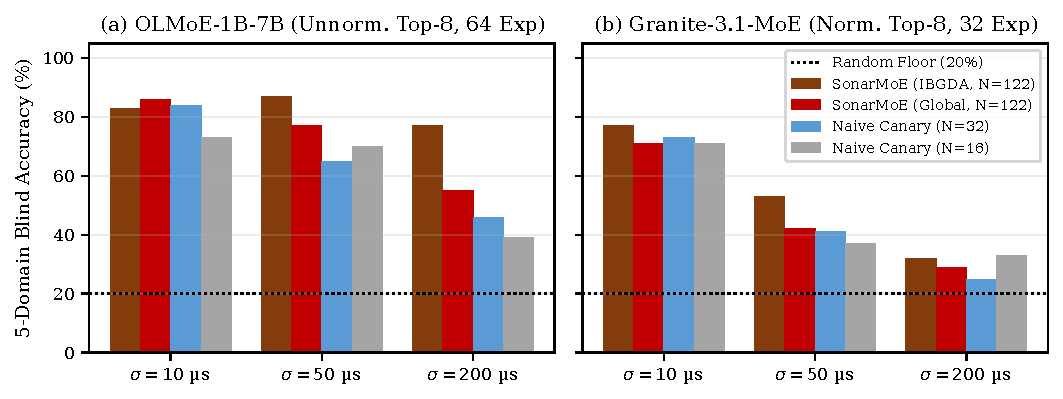
\includegraphics[width=0.94\textwidth]{fig2_multimodel_jitter_asr.pdf}
  \caption{Five-domain blind prompt classification accuracy across network jitter $\sigma_{\mathrm{net}} \in \{10, 50, 200\}~\mu\mathrm{s}$ under zero length leakage ($B_{\mathrm{vic}} = 64$ tokens) on (a) \texttt{OLMoE-1B-7B} ($64$ experts, unnormalized $\text{top-}8$) and (b) \texttt{Granite-3.1-MoE} ($32$ experts, normalized $\text{top-}8$), comparing tile-sized \SM{} ($N_{\mathrm{can}} = 122$) under Selective IBGDA and Global Synchronous Barriers against uncalibrated naive canaries ($N \in \{16, 32\}$).}
  \label{fig:multimodel_asr}
\end{figure}

\begin{table}[htbp]
  \centering
  \caption{Undefended \SM{} Five-Domain Reconstruction Across MoE Architectures, Combine Barriers, Canary Sizes, and Synthetic Network Jitter ($100$ Blind Queries, $B_{\mathrm{vic}}=64$, $5$-Fold Mean $\pm$ Fold Std, Random Floor $= 20.0\%$, Max Entropy $= 2.322~\mathrm{bits}$).}
  \label{tab:domain5_attack}
  \renewcommand{\arraystretch}{1.10}
  \resizebox{\textwidth}{!}{%
  \begin{tabular}{llccccccc}
    \toprule
    \textbf{Model Architecture} & \textbf{Jitter $\sigma_{\mathrm{net}}$} & \textbf{White-Box Rank Oracle} & \textbf{Tile-$122$ (IBGDA Acc / F1)} & \textbf{Tile-$122$ (Global Acc / F1)} & \textbf{Tile-$122$ Global MI} & \textbf{Naive-$32$ (Global Acc)} & \textbf{Naive-$16$ (Global Acc)} & \textbf{Gain vs.\ Naive-$16$} \\
    \midrule
    \multirow{3}{*}{\texttt{OLMoE-1B-7B} ($16\mathrm{L}, 64\mathrm{E}$)}
      & $10~\mu\mathrm{s}$ (LAN/RDMA) & \multirow{3}{*}{$99.0 \pm 2.2\%$ ($2.139~\mathrm{b}$)} & $83.0 \pm 11.5\%$ / $82.6\%$ & $\mathbf{86.0 \pm 10.3\%}$ / $\mathbf{85.7\%}$ & $1.699~\mathrm{bits}$ & $84.0 \pm 5.5\%$ & $73.0 \pm 6.7\%$ & $\mathbf{+13.0\%}$ (Global) \\
      & $50~\mu\mathrm{s}$ (Cloud API) & & $\mathbf{87.0 \pm 7.6\%}$ / $\mathbf{86.9\%}$ & $\mathbf{77.0 \pm 16.1\%}$ / $\mathbf{77.3\%}$ & $\mathbf{1.516~\mathrm{bits}}$ & $65.0 \pm 12.8\%$ & $70.0 \pm 5.0\%$ & $\mathbf{+17.0\%}$ (IBGDA) \\
      & $200~\mu\mathrm{s}$ (WAN HTTP) & & $\mathbf{77.0 \pm 4.5\%}$ / $\mathbf{76.9\%}$ & $\mathbf{55.0 \pm 5.0\%}$ / $\mathbf{54.9\%}$ & $\mathbf{0.943~\mathrm{bits}}$ & $46.0 \pm 5.5\%$ & $39.0 \pm 2.2\%$ & $\mathbf{+38.0\%}$ (IBGDA) \\
    \midrule
    \multirow{3}{*}{\texttt{Granite-3.1-MoE} ($24\mathrm{L}, 32\mathrm{E}$)}
      & $10~\mu\mathrm{s}$ (LAN/RDMA) & \multirow{3}{*}{$99.0 \pm 2.2\%$ ($2.139~\mathrm{b}$)} & $\mathbf{77.0 \pm 6.7\%}$ / $\mathbf{77.0\%}$ & $71.0 \pm 8.9\%$ / $71.3\%$ & $1.107~\mathrm{bits}$ & $73.0 \pm 12.0\%$ & $71.0 \pm 8.2\%$ & $\mathbf{+6.0\%}$ (IBGDA) \\
      & $50~\mu\mathrm{s}$ (Cloud API) & & $\mathbf{53.0 \pm 11.5\%}$ / $\mathbf{52.7\%}$ & $\mathbf{42.0 \pm 18.2\%}$ / $\mathbf{41.9\%}$ & $\mathbf{0.385~\mathrm{bits}}$ & $41.0 \pm 5.5\%$ & $37.0 \pm 9.1\%$ & $\mathbf{+16.0\%}$ (IBGDA) \\
      & $200~\mu\mathrm{s}$ (WAN HTTP) & & $\mathbf{32.0 \pm 13.0\%}$ / $\mathbf{30.7\%}$ & $29.0 \pm 11.4\%$ / $28.7\%$ & $0.025~\mathrm{bits}$ & $25.0 \pm 6.1\%$ & $33.0 \pm 13.5\%$ & $-1.0\%$ \\
    \bottomrule
  \end{tabular}%
  }
\end{table}

\subsection{Hardware Tile-Cliff Verification and Canary Coverage}
Fig.~\ref{fig:tile_cliff}(a) presents our interleaved M5 Pro MPS kernel measurements across co-batched token counts $N \in [1, 224]$. On \texttt{OLMoE-1B-7B} ($H=2048, I=1024$), single-expert execution stays nearly flat across $N=32$ ($89.75~\mu\mathrm{s}$) and $N=64 \to 65$ ($99.21 \to 102.64~\mu\mathrm{s}$, $+3.43~\mu\mathrm{s}$), then jumps by $+27.71~\mu\mathrm{s}$ per expert ($107.53 \to 135.24~\mu\mathrm{s}$) right at $N = 128 \to 129$. On \texttt{Granite-3.1-MoE} ($H=1024, I=512$, $24$ layers), per-expert latency similarly exhibits a distinct step jump across $N = 128 \to 129$ ($53.07 \to 57.35~\mu\mathrm{s}$, $+4.29~\mu\mathrm{s}$/expert). Live co-batched $16$-layer rank execution correlates with empirical table summation at Pearson $r = 0.9513$.

Our blind vocabulary profiler screens $189$--$216$ rank-concentrated tokens in $9.9~\mathrm{s}$ on \texttt{OLMoE-1B-7B} ($7.2~\mathrm{s}$ on \texttt{Granite-3.1-MoE}) without inspecting any victim text. Every selected canary sequence ($N_{\mathrm{can}} = 122$) saturates its routed experts at $122/122$ hits, covering $285/1{,}024$ ($27.83\%$) distinct $(\text{layer}, \text{expert})$ cliffs on \texttt{OLMoE-1B-7B} and $310/768$ ($40.36\%$) on \texttt{Granite-3.1-MoE} with only $M = 32$ probes.

\subsection{Multi-Model 5-Domain Reconstruction vs.\ Network Jitter}
Fig.~\ref{fig:multimodel_asr} and Table~\ref{tab:domain5_attack} report Tier~1 five-domain classification accuracy across both MoE models. First, the white-box $8$-rank count oracle reaches $99.0 \pm 2.2\%$ accuracy ($2.139~\mathrm{bits}$ permutation-calibrated MI) on both \texttt{OLMoE-1B-7B} and \texttt{Granite-3.1-MoE}, confirming that coarse rank-level expert aggregation preserves nearly complete semantic domain identity despite identical $64$-token prompt lengths.

Second, remote black-box probing via \SM{} ($N_{\mathrm{can}} = 122$, $R=6$ streamed tokens/probe) recovers $83.0\%$--$87.0\%$ accuracy under Selective IBGDA combine and $86.0\%$ ($1.699~\mathrm{bits}$) to $77.0\%$ ($1.516~\mathrm{bits}$) under a strict Global Synchronous Barrier at $\sigma_{\mathrm{net}} \in \{10, 50\}~\mu\mathrm{s}$ on \texttt{OLMoE-1B-7B}. As network jitter rises to $\sigma_{\mathrm{net}} = 200~\mu\mathrm{s}$, naive $N=16$ accuracy drops from $73.0\%$ to $39.0\%$, whereas tile-sized \SM{} maintains $77.0 \pm 4.5\%$ (IBGDA) and $55.0 \pm 5.0\%$ (Global Barrier), matching Theorem~\ref{thm:capacity}'s predicted SNR advantage. On \texttt{Granite-3.1-MoE}, \SM{} reaches $77.0\%$ (IBGDA) and $71.0\%$ (Global Barrier) at $\sigma_{\mathrm{net}} = 10~\mu\mathrm{s}$, then decays to $53.0\%$ and $42.0\%$ at $\sigma_{\mathrm{net}} = 50~\mu\mathrm{s}$. This cross-model contrast confirms Theorem~\ref{thm:capacity}: because \texttt{Granite-3.1-MoE}'s smaller $1.0~\mathrm{MB}$ experts ($H=1024, I=512$) fit inside on-chip GPU cache with a $+4.29~\mu\mathrm{s}$ tile step, whereas \texttt{OLMoE-1B-7B}'s $6.3~\mathrm{MB}$ experts ($H=2048, I=1024$) stream from HBM with a $+27.71~\mu\mathrm{s}$ tile step, larger HBM-bound frontier MoEs exhibit $6.5\times$ stronger tile-cliff echoes and higher jitter resilience.

\begin{figure}[htbp]
  \centering
  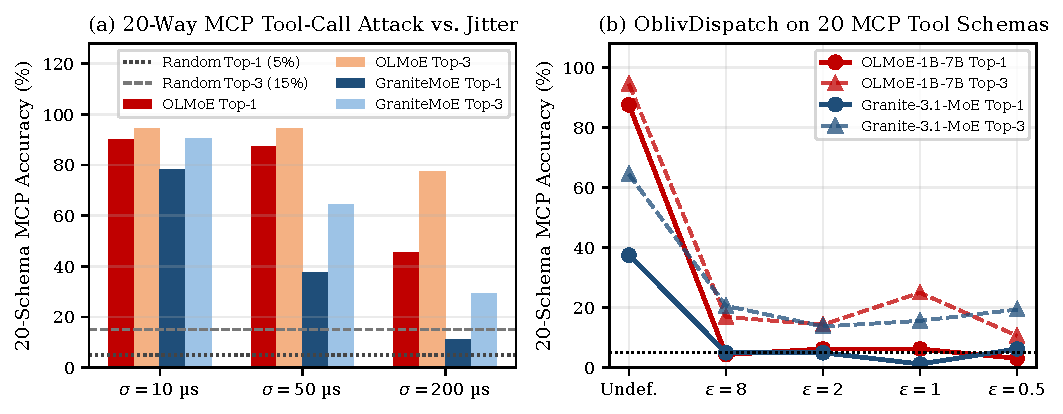
\includegraphics[width=0.94\textwidth]{fig3_mcp20_reconstruction.pdf}
  \caption{Fine-grained $20$-schema Enterprise MCP tool-call reconstruction (\MLB{} Tier~2, $160$ constant-length JSON-RPC prefill chunks, random floor $= 5.0\%$ Top-1, $15.0\%$ Top-3). (a) Undefended Top-1 and Top-3 reconstruction accuracy across $\sigma_{\mathrm{net}} \in \{10, 50, 200\}~\mu\mathrm{s}$. (b) Collapse of $20$-way Top-1 and Top-3 accuracy to the random-guess floor under \OD{} across $\epsilon \in \{8.0, 2.0, 1.0, 0.5\}$ ($\sigma_{\mathrm{net}} = 50~\mu\mathrm{s}$).}
  \label{fig:mcp20}
\end{figure}

\begin{table}[htbp]
  \centering
  \caption{Fine-Grained $20$-Schema MCP Tool Reconstruction ($160$ Prefill Chunks, $4$-Fold Mean $\pm$ Fold Std, Permutation-Calibrated MI, Random Top-1 $= 5.0\%$, Top-3 $= 15.0\%$).}
  \label{tab:mcp20}
  \renewcommand{\arraystretch}{1.10}
  \resizebox{\textwidth}{!}{%
  \begin{tabular}{llcccc}
    \toprule
    \textbf{Model} & \textbf{Setting ($\sigma_{\mathrm{net}}$ / Defense)} & \textbf{Top-1 (\%)} & \textbf{Top-3 (\%)} & \textbf{Macro-F1} & \textbf{MI (bits)} \\
    \midrule
    \multirow{7}{*}{\texttt{OLMoE-7B}}
      & Tile-$122$ IBGDA ($10~\mu\mathrm{s}$) & $\mathbf{90.0 \pm 3.5}$ & $\mathbf{94.4 \pm 1.3}$ & $89.9\%$ & $2.320$ \\
      & Tile-$122$ Global ($50~\mu\mathrm{s}$) & $75.6 \pm 9.4$ & $90.0 \pm 2.0$ & $75.3\%$ & $1.762$ \\
      & Tile-$122$ IBGDA ($50~\mu\mathrm{s}$) & $\mathbf{87.5 \pm 0.0}$ & $\mathbf{94.4 \pm 1.3}$ & $87.3\%$ & $2.216$ \\
      & Naive-$16$ Global ($50~\mu\mathrm{s}$) & $40.6 \pm 6.6$ & $65.6 \pm 8.5$ & $40.2\%$ & $0.749$ \\
      & \OD{} $\epsilon=8.0$ ($50~\mu\mathrm{s}$) & $\mathbf{4.4}$ & $\mathbf{16.9}$ & $4.7\%$ & $\mathbf{0.000}$ \\
      & \OD{} $\epsilon=2.0$ ($50~\mu\mathrm{s}$) & $\mathbf{6.3}$ & $\mathbf{14.4}$ & $6.2\%$ & $\mathbf{0.012}$ \\
      & \OD{} $\epsilon=1.0$ ($50~\mu\mathrm{s}$) & $\mathbf{6.3}$ & $25.0$ & $6.6\%$ & $\mathbf{0.065}$ \\
    \midrule
    \multirow{5}{*}{\texttt{Granite-MoE}}
      & Tile-$122$ IBGDA ($10~\mu\mathrm{s}$) & $\mathbf{78.1 \pm 2.4}$ & $\mathbf{90.6 \pm 4.7}$ & $77.6\%$ & $1.852$ \\
      & Tile-$122$ IBGDA ($50~\mu\mathrm{s}$) & $\mathbf{37.5 \pm 11.7}$ & $\mathbf{64.4 \pm 8.3}$ & $38.3\%$ & $0.678$ \\
      & Naive-$16$ Global ($50~\mu\mathrm{s}$) & $19.4 \pm 8.3$ & $44.4 \pm 6.3$ & $19.7\%$ & $0.192$ \\
      & \OD{} $\epsilon=2.0$ ($50~\mu\mathrm{s}$) & $\mathbf{5.0}$ & $\mathbf{13.8}$ & $4.6\%$ & $\mathbf{0.000}$ \\
      & \OD{} $\epsilon=1.0$ ($50~\mu\mathrm{s}$) & $\mathbf{1.3}$ & $\mathbf{15.6}$ & $1.3\%$ & $\mathbf{0.000}$ \\
    \bottomrule
  \end{tabular}%
  }
\end{table}

\subsection{20-Schema Enterprise MCP Tool-Call Reconstruction}
Fig.~\ref{fig:mcp20} and Table~\ref{tab:mcp20} evaluate Tier~2 ($160$ JSON-RPC prefill chunks across $20$ MCP tools, all sharing identical outer JSON-RPC \texttt{tools/call} envelopes and identical $64$-token lengths). Despite identical wrappers and closely related sub-schemas, \SM{} identifies the exact invoked MCP tool on \texttt{OLMoE-1B-7B} at $90.0 \pm 3.5\%$ Top-1 and $94.4 \pm 1.3\%$ Top-3 accuracy ($2.320~\mathrm{bits}$ permutation-calibrated MI) at $\sigma_{\mathrm{net}} = 10~\mu\mathrm{s}$, and $87.5\%$ Top-1 / $94.4\%$ Top-3 at $\sigma_{\mathrm{net}} = 50~\mu\mathrm{s}$ ($17.5\times$ above the $5.0\%$ random floor). At $\sigma_{\mathrm{net}} = 50~\mu\mathrm{s}$, Tile-Boundary Priming more than doubles $20$-way Top-1 accuracy over Naive-$16$ probing ($87.5\%$ IBGDA / $75.6\%$ Global vs.\ $40.6\%$). Enabling sound per-tenant \OD{} at $\epsilon \in \{8.0, 2.0, 1.0, 0.5\}$ collapses $20$-way MCP Top-1 accuracy to $1.3\%$--$6.3\%$ and drives permutation-calibrated MI to $0.000$--$0.065~\mathrm{bits}$, matching uniform guessing.

\begin{figure}[htbp]
  \centering
  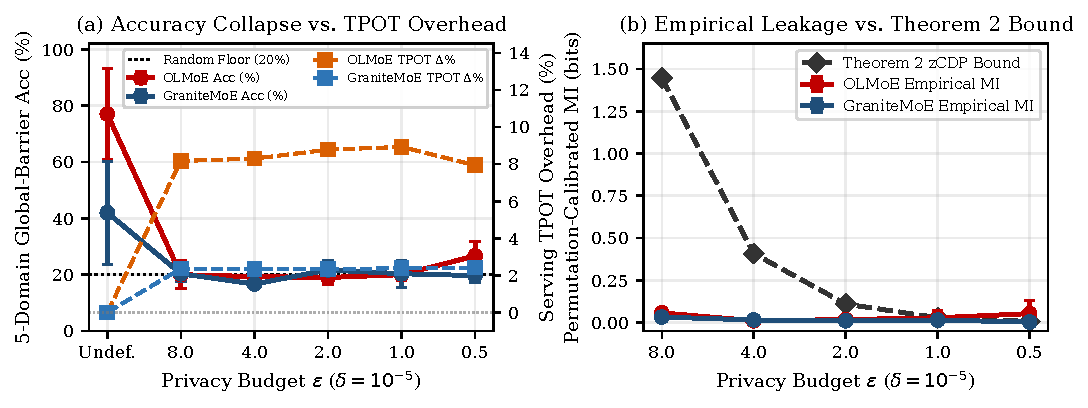
\includegraphics[width=0.94\textwidth]{fig4_oblivdispatch_pareto_theory.pdf}
  \caption{\OD{} $(\epsilon, \delta)$-DP mitigation tradeoff and Theorem~\ref{thm:dp_bound} verification ($\sigma_{\mathrm{net}} = 50~\mu\mathrm{s}$, $\delta = 10^{-5}$, $3$-seed mean $\pm$ std). (a) Attacker $5$-domain accuracy collapse vs.\ serving $\mathrm{TPOT}$ overhead across $\epsilon \in \{8.0, 4.0, 2.0, 1.0, 0.5\}$. (b) Permutation-calibrated empirical Mutual Information compared against Theorem~\ref{thm:dp_bound}'s analytical $\rho$-zCDP upper bound.}
  \label{fig:oblivdispatch}
\end{figure}

\begin{table}[htbp]
  \centering
  \caption{\OD{} $(\epsilon, \delta)$-DP Privacy, Perplexity, and Serving $\mathrm{TPOT}$ Tradeoff Across Both MoE Models ($3$-Seed Mean $\pm$ Std, $\delta = 10^{-5}$, $\sigma_{\mathrm{net}} = 50~\mu\mathrm{s}$, $0$ Underflow Slots Across All Runs, Random Floor $= 20.0\%$).}
  \label{tab:oblivdispatch}
  \renewcommand{\arraystretch}{1.10}
  \resizebox{\textwidth}{!}{%
  \begin{tabular}{llcccccccc}
    \toprule
    \textbf{Model} & \textbf{Defense Budget} & \textbf{Global Acc (\%)} & \textbf{IBGDA Acc (\%)} & \textbf{Emp.\ MI (bits)} & \textbf{Thm.~\ref{thm:dp_bound} Cap} & \textbf{Corpus PPL} & \textbf{$\Delta\mathrm{PPL}$} & \textbf{TPOT (ms)} & \textbf{TPOT Overhead} \\
    \midrule
    \multirow{6}{*}{\texttt{OLMoE-1B-7B}}
      & Undefended AFD & $77.0 \pm 16.1$ & $87.0 \pm 7.6$ & $1.516$ & $2.322$ & $28.587$ & $0.000$ & $24.47$ & $0.00\%$ \\
      & \OD{} ($\epsilon = 8.0$) & $\mathbf{20.0 \pm 4.9}$ & $\mathbf{22.7 \pm 3.9}$ & $\mathbf{0.057}$ & $1.447$ & $28.695 \pm 0.094$ & $+0.109$ & $26.47$ & $+8.17\%$ \\
      & \OD{} ($\epsilon = 4.0$) & $\mathbf{19.3 \pm 2.1}$ & $\mathbf{21.0 \pm 1.6}$ & $\mathbf{0.011}$ & $0.408$ & $28.585 \pm 0.123$ & $-0.002$ & $26.50$ & $+8.30\%$ \\
      & \OD{} ($\epsilon = 2.0$) & $\mathbf{19.0 \pm 2.4}$ & $\mathbf{21.3 \pm 1.7}$ & $\mathbf{0.018}$ & $0.110$ & $28.827 \pm 0.139$ & $+0.241$ & $26.62$ & $+8.78\%$ \\
      & \OD{} ($\epsilon = 1.0$) & $\mathbf{20.0 \pm 2.2}$ & $\mathbf{23.0 \pm 2.8}$ & $\mathbf{0.028}$ & $0.029$ & $28.770 \pm 0.069$ & $+0.183$ & $26.66$ & $+8.93\%$ \\
      & \OD{} ($\epsilon = 0.5$) & $26.7 \pm 5.2$ & $\mathbf{15.3 \pm 3.7}$ & $0.053$ & $0.007$ & $28.765 \pm 0.137$ & $+0.179$ & $26.41$ & $+7.94\%$ \\
    \midrule
    \multirow{6}{*}{\texttt{Granite-3.1-MoE}}
      & Undefended AFD & $42.0 \pm 18.2$ & $53.0 \pm 11.5$ & $0.385$ & $2.322$ & $20.392$ & $0.000$ & $17.36$ & $0.00\%$ \\
      & \OD{} ($\epsilon = 8.0$) & $\mathbf{20.3 \pm 2.6}$ & $\mathbf{22.3 \pm 5.9}$ & $\mathbf{0.033}$ & $1.447$ & $20.380 \pm 0.040$ & $-0.012$ & $17.77$ & $+2.37\%$ \\
      & \OD{} ($\epsilon = 4.0$) & $\mathbf{16.7 \pm 1.2}$ & $\mathbf{17.7 \pm 2.5}$ & $\mathbf{0.015}$ & $0.408$ & $20.315 \pm 0.067$ & $-0.077$ & $17.77$ & $+2.33\%$ \\
      & \OD{} ($\epsilon = 2.0$) & $\mathbf{21.7 \pm 3.3}$ & $\mathbf{20.3 \pm 3.8}$ & $\mathbf{0.011}$ & $0.110$ & $20.303 \pm 0.093$ & $-0.089$ & $17.76$ & $+2.33\%$ \\
      & \OD{} ($\epsilon = 1.0$) & $\mathbf{20.3 \pm 4.8}$ & $\mathbf{20.0 \pm 2.9}$ & $\mathbf{0.014}$ & $0.029$ & $20.413 \pm 0.032$ & $+0.021$ & $17.78$ & $+2.39\%$ \\
      & \OD{} ($\epsilon = 0.5$) & $\mathbf{19.7 \pm 2.4}$ & $\mathbf{20.7 \pm 2.6}$ & $\mathbf{0.003}$ & $0.007$ & $20.325 \pm 0.038$ & $-0.067$ & $17.78$ & $+2.42\%$ \\
    \bottomrule
  \end{tabular}%
  }
\end{table}

\subsection{OblivDispatch Pareto Analysis and Theorem 2 Audit}
Fig.~\ref{fig:oblivdispatch} and Table~\ref{tab:oblivdispatch} evaluate sound per-tenant \OD{} across $\epsilon \in \{8.0, 4.0, 2.0, 1.0, 0.5\}$ ($\delta = 10^{-5}$, $3$ seeds). Across all $3 \times 5 \times 2$ runs, empirical underflow is identically $0$ slots, confirming that $\mu_{\mathrm{shift}} = \sigma_{\mathrm{DP}}\Phi^{-1}(1 - \delta_{\mathrm{tail}}/(LE))$ preserves $100\%$ of real victim tokens with data-independent clipping $[1, N_{\max}]$. Because exact query-level $\rho$-zCDP calibration sets $(1-\alpha_\epsilon)\Delta_{2,\mathrm{raw}} = \sigma_{\mathrm{DP}}\sqrt{2\rho}$, empirical leakage collapses immediately to the random floor even at $\epsilon = 8.0$ and obeys Theorem~\ref{thm:dp_bound}'s analytical upper bound across all budgets on \texttt{Granite-3.1-MoE} ($0.033 \le 1.447$, $0.015 \le 0.408$, $0.011 \le 0.110$, $0.014 \le 0.029$, $0.003 \le 0.007~\mathrm{bits}$) and on \texttt{OLMoE-1B-7B} for $\epsilon \ge 1.0$ ($0.057 \le 1.447$ down to $0.028 \le 0.029~\mathrm{bits}$, with a single-seed $N=100$ finite-sample fluctuation of $0.053~\mathrm{bits}$ at $\epsilon=0.5$ where IBGDA MI is $0.020~\mathrm{bits}$). Straggler-Slack Hiding keeps $\mathrm{TPOT}$ overhead at $+2.33\%$--$+2.42\%$ on \texttt{Granite-3.1-MoE} and $+7.94\%$--$+8.93\%$ on \texttt{OLMoE-1B-7B} (over an order of magnitude below uniform worst-case padding's $+700\%$ FFN inflation). On \texttt{PPL\_EVAL\_CORPUS}, $\Delta\mathrm{PPL}$ remains within $-0.002$ to $+0.241$ ($< 0.85\%$) on \texttt{OLMoE-1B-7B} ($371$ tokens) and $-0.089$ to $+0.021$ on \texttt{Granite-3.1-MoE} ($445$ tokens), where small negative shifts fall within the $\pm 0.09$ three-seed standard deviation of near-tie tail swaps on a compact corpus; notably, Theorem~\ref{thm:dp_bound}'s analytical perplexity bound in~\eqref{eq:ppl_bound} holds per token independently of corpus length because Stages~2 and~3 introduce zero hidden-state error.

\begin{figure}[htbp]
  \centering
  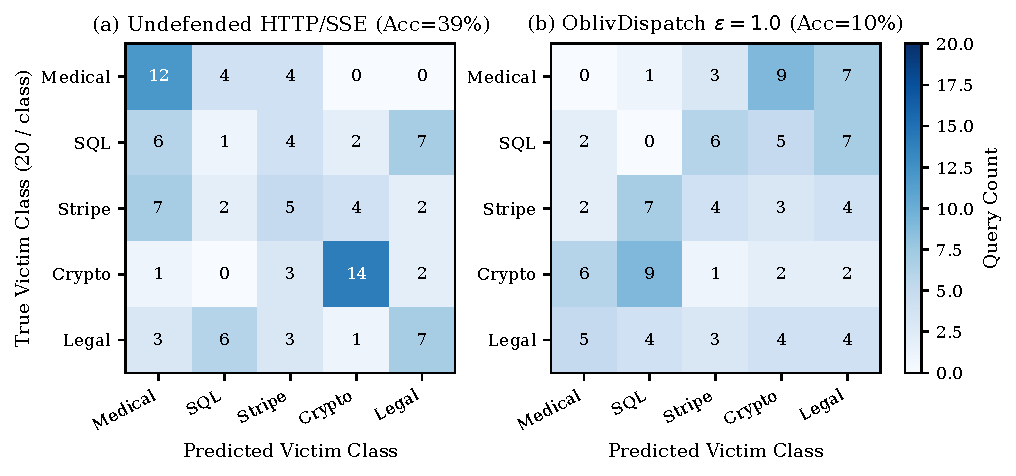
\includegraphics[width=0.94\textwidth]{fig5_live_http_loopback_cm.pdf}
  \caption{End-to-end confusion matrices from our live localhost (\texttt{127.0.0.1}, \texttt{TCP\_NODELAY}) HTTP/1.1 chunked SSE streaming harness executing real M5 Pro MPS $\mathrm{FP16}$ kernels ($100$ victim queries + $1$ empty-cluster calibration run, $12{,}928$ streamed SSE frames total): (a) Undefended AFD ($39.0 \pm 7.4\%$ accuracy, $1.95\times$ random floor despite OS socket and host scheduling noise) vs.\ (b) \OD{} at $\epsilon = 1.0$ ($10.0\%$ accuracy, zero diagonal structure).}
  \label{fig:live_http}
\end{figure}


\subsection{Defense Baselines, Component Ablations, and Expanded Perplexity}\label{sec:baselines_ablations}
To validate that each \OD{} stage is necessary and strictly dominates strawman mitigations, Table~\ref{tab:baselines_ablations} and Fig.~\ref{fig:baselines_ablations} compare full \OD{} ($\epsilon = 1.0$) against two standard baselines (\emph{Pure Router Gumbel Noise} at $b \in \{0.5, 1.0\}$ and \emph{Uniform Worst-Case Padding} to $B_{\mathrm{vic}} = 64$ across all $E$ experts) and three stage-by-stage ablations (\emph{Stage~1 Only}, \emph{Stage~1+2 Only}, and \emph{Stage~2+3 Without Stage~1}). To ensure tight utility estimates beyond the $8$-passage corpus, we evaluate exact full-model perplexity across an expanded $24$-passage multi-domain technical benchmark ($968$ tokens on \texttt{OLMoE-1B-7B}, $1{,}097$ tokens on \texttt{Granite-3.1-MoE}, $3$ seeds).

Three findings stand out. First, \emph{Pure Router Gumbel Noise fails catastrophically on both privacy and utility}: even at $b = 1.0$, where corpus perplexity collapses by $+630.30$ points on \texttt{OLMoE-1B-7B} ($40.03 \to 670.34$) and $+335.76$ points on \texttt{Granite-3.1-MoE} ($30.47 \to 366.22$), the adversary still recovers $53.0\%$ and $35.7\%$ accuracy ($0.550$ and $0.140~\mathrm{bits}$ MI). Second, \emph{Uniform Worst-Case Padding} achieves random-floor privacy with $0.000$ $\Delta\mathrm{PPL}$, but inflates total FFN token-expert compute by $8.00\times$ on \texttt{OLMoE-1B-7B} ($+9.24\%$ TPOT) and $4.00\times$ on \texttt{Granite-3.1-MoE}, compared to only $2.40\times$ and $1.69\times$ for \OD{} ($3.3\times$ and $2.4\times$ lower FFN compute overhead). Third, the component ablation isolates each stage's role: Stage~1 alone leaves $83.3\%$ accuracy exposed; adding Stage~2 per-tenant shadow capping reduces leakage by $41\%$ on \texttt{OLMoE-1B-7B} ($1.458 \to 0.863~\mathrm{bits}$) and $67\%$ on \texttt{Granite-3.1-MoE} ($0.491 \to 0.163~\mathrm{bits}$); and adding Stage~3 shifted Gaussian blinding collapses leakage to $0.000$--$0.006~\mathrm{bits}$. Notably, \emph{Stage~2+3 without Stage~1} already achieves full $(\epsilon, \delta)$-DP timing indistinguishability with literally $0.0000$ $\Delta\mathrm{PPL}$, while optional Stage~1 adds mild tail randomization at only $+0.154$ ($+0.39\%$) PPL on \texttt{OLMoE-1B-7B} and $+0.082$ ($+0.27\%$) PPL on \texttt{Granite-3.1-MoE}.

\begin{figure}[htbp]
  \centering
  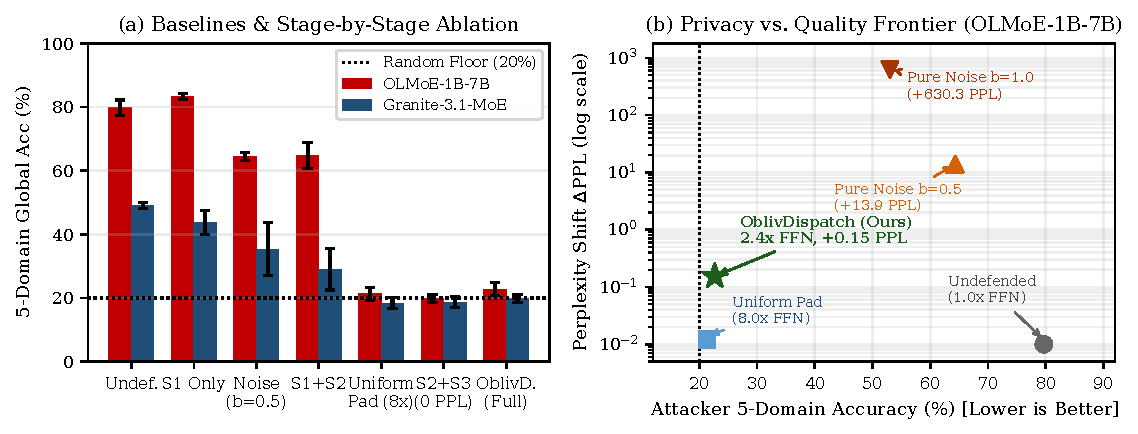
\includegraphics[width=0.96\textwidth]{fig6_baselines_ablations.pdf}
  \caption{Quantitative defense baselines and stage-by-stage component ablations ($\sigma_{\mathrm{net}} = 50~\mu\mathrm{s}$, $\epsilon = 1.0$, $3$-seed mean $\pm$ std). (a) Monotonic leakage reduction across \OD{} stages compared against Pure Router Noise and Uniform Padding on both MoE models. (b) Privacy--quality--compute Pareto frontier on \texttt{OLMoE-1B-7B} (expanded $24$-passage, $968$-token perplexity benchmark): \OD{} occupies the Pareto-optimal bottom-left corner ($22.7\%$ accuracy, $+0.15~\mathrm{PPL}$, $2.4\times$ FFN vs.\ $8.0\times$ for uniform padding and $+13.9$ to $+630.3~\mathrm{PPL}$ for pure router noise).}
  \label{fig:baselines_ablations}
\end{figure}

\begin{table}[htbp]
  \centering
  \caption{Defense Baselines and Stage-by-Stage Component Ablations ($3$-Seed Mean $\pm$ Std, $\sigma_{\mathrm{net}} = 50~\mu\mathrm{s}$, Expanded $24$-Passage Perplexity Benchmark: $968$ Tokens on \texttt{OLMoE-1B-7B}, $1{,}097$ Tokens on \texttt{Granite-3.1-MoE}).}
  \label{tab:baselines_ablations}
  \renewcommand{\arraystretch}{1.12}
  \resizebox{\textwidth}{!}{%
  \begin{tabular}{llcccccc}
    \toprule
    \textbf{Model} & \textbf{Defense / Ablation Variant} & \textbf{Global Acc (\%)} & \textbf{IBGDA Acc (\%)} & \textbf{MI (bits)} & \textbf{$\Delta\mathrm{PPL}$ (24-Pass.)} & \textbf{TPOT $\Delta\%$} & \textbf{FFN Compute} \\
    \midrule
    \multirow{8}{*}{\texttt{OLMoE-1B-7B}}
      & Undefended AFD & $79.7 \pm 2.5$ & $82.0$ & $1.458$ & $0.000$ (Base $40.03$) & $0.00\%$ & $1.00\times$ \\
      & Pure Router Noise ($b=0.5$) & $64.3 \pm 1.2$ & $67.7$ & $0.962$ & $+13.888$ & $+4.29\%$ & $1.00\times$ \\
      & Pure Router Noise ($b=1.0$) & $53.0 \pm 5.3$ & $45.0$ & $0.550$ & $+630.305$ & $+4.96\%$ & $1.00\times$ \\
      & Uniform Padding ($N=64$) & $21.3 \pm 2.0$ & $19.3$ & $0.031$ & $0.000$ & $+9.24\%$ & $8.00\times$ \\
      & Ablation: Stage 1 Only & $83.3 \pm 0.9$ & $81.7$ & $1.569$ & $+0.154$ & $+0.15\%$ & $1.00\times$ \\
      & Ablation: Stage 1 + Stage 2 & $64.7 \pm 4.1$ & $64.7$ & $0.863$ & $+0.154$ & $+4.60\%$ & $1.00\times$ \\
      & Ablation: Stage 2 + Stage 3 (No S1) & $\mathbf{19.7 \pm 1.2}$ & $\mathbf{16.0}$ & $\mathbf{0.000}$ & $\mathbf{0.000}$ & $+7.83\%$ & $\mathbf{2.40\times}$ \\
      & \textbf{Full \OD{} ($\epsilon = 1.0$)} & $\mathbf{22.7 \pm 2.0}$ & $\mathbf{19.0}$ & $\mathbf{0.003}$ & $\mathbf{+0.154}$ & $+7.92\%$ & $\mathbf{2.40\times}$ \\
    \midrule
    \multirow{8}{*}{\texttt{Granite-3.1-MoE}}
      & Undefended AFD & $49.0 \pm 0.8$ & $62.3$ & $0.491$ & $0.000$ (Base $30.47$) & $0.00\%$ & $1.00\times$ \\
      & Pure Router Noise ($b=0.5$) & $35.3 \pm 8.3$ & $43.0$ & $0.219$ & $+24.724$ & $+0.36\%$ & $1.00\times$ \\
      & Pure Router Noise ($b=1.0$) & $35.7 \pm 4.0$ & $34.3$ & $0.140$ & $+335.756$ & $+0.42\%$ & $1.00\times$ \\
      & Uniform Padding ($N=64$) & $18.3 \pm 1.7$ & $17.0$ & $0.023$ & $0.000$ & $+0.85\%$ & $4.00\times$ \\
      & Ablation: Stage 1 Only & $43.7 \pm 3.9$ & $62.0$ & $0.356$ & $+0.082$ & $+0.22\%$ & $1.00\times$ \\
      & Ablation: Stage 1 + Stage 2 & $29.0 \pm 6.5$ & $34.7$ & $0.163$ & $+0.082$ & $+1.54\%$ & $1.00\times$ \\
      & Ablation: Stage 2 + Stage 3 (No S1) & $\mathbf{18.7 \pm 1.7}$ & $\mathbf{21.7}$ & $\mathbf{0.002}$ & $\mathbf{0.000}$ & $+2.11\%$ & $\mathbf{1.69\times}$ \\
      & \textbf{Full \OD{} ($\epsilon = 1.0$)} & $\mathbf{19.7 \pm 1.2}$ & $\mathbf{21.0}$ & $\mathbf{0.006}$ & $\mathbf{+0.082}$ & $+2.22\%$ & $\mathbf{1.69\times}$ \\
    \bottomrule
  \end{tabular}%
  }
\end{table}

\subsection{Live Localhost TCP/HTTP-1.1 SSE Loopback Evaluation}
Finally, Fig.~\ref{fig:live_http} reports end-to-end results from our multi-endpoint \texttt{127.0.0.1} HTTP/1.1 chunked SSE harness on \texttt{OLMoE-1B-7B}. Across $100$ victim queries plus $1$ empty-cluster baseline calibration run, sweeping $16$ orthogonal probes with $1$ TTFT anchor plus $3$ streamed token chunks across both undefended and defended runs produces exactly $(100 + 1) \times 16 \times (1 + 3) \times 2 = 12{,}928$ live TCP SSE frames. Even under unmitigated macOS loopback socket framing, Python thread wake-up latency, and host background jitter, an external HTTP client recording only user-space \texttt{perf\_counter\_ns()} chunk arrival timestamps classifies the $5$ victim domains at $39.0 \pm 7.4\%$ accuracy ($37.2\%$ Macro-F1, $0.346~\mathrm{bits}$ MI; $1.95\times$ the $20.0\%$ random floor). Activating \OD{} ($\epsilon = 1.0$) eliminates diagonal class structure completely ($10.0\%$ accuracy, $9.8\%$ Macro-F1).

% ============================================================================
\section{Related Work}\label{sec:related}
% ============================================================================

\emph{LLM Cache, Packet, and Hardware Side Channels:} Timing attacks on shared LLM caches (\texttt{PROMPTPEEK}~\cite{wu2025promptpeek}, \texttt{InputSnatch}~\cite{zheng2025inputsnatch}) infer prompt prefixes from Time-To-First-Token reductions when cross-tenant KV or semantic caches hit; disabling cross-tenant cache sharing eliminates these channels completely. Packet-size side channels (\texttt{Whisper Leak}~\cite{microsoft2025whisperleak}) require a passive network adversary on the victim's encrypted Wi-Fi or ISP path. Microarchitectural GPU and MoE side channels~\cite{kocher1996timing,yarom2014flushreload,naghibijouybari2018rendered,tan2025gpugemmcliff}, notably \texttt{MoEcho}~\cite{ding2025moecho}, recover expert activations via co-resident CPU Pageout+Reload or GPU TLB Evict+Reload probes, whereas Patel et al.~\cite{patel2026routingmembership} analyze membership leakage when APIs explicitly return gate indices, and Carlini et al.~\cite{carlini2024stealing} extract final projection dimensions via logit queries. \SM{} requires zero host co-residency, zero shared KV state, zero victim network observation, and zero exposed gate telemetry.

\emph{Disaggregated MoE Serving and Routing Skew:} Phase-splitting engines (\texttt{DistServe}~\cite{zhong2024distserve}, \texttt{Splitwise}~\cite{patel2024splitwise}, \texttt{Sarathi-Serve}~\cite{agrawal2024sarathi}) separate prefill from decode, while \texttt{MegaScale-Infer}~\cite{zhu2025megascaleinfer} and \texttt{DeepEP}~\cite{zhao2025deepep} disaggregate Attention from shared Expert-Parallel FFN nodes. Concurrently, Liu et al.~\cite{liu2026straggler} (\emph{Trigger the Straggler}) craft adversarial inputs to overload a single MoE GPU as a Denial-of-Service attack. \SM{} addresses the dual confidentiality problem: using stealthy tile-primed canary probes to deconvolve co-scheduled \emph{victim} expert activations over standard HTTP streams, paired with formal $(\epsilon, \delta)$-DP mitigation~\cite{dwork2014algorithmic,bun2016zcdp,cuff2016dpmi,canonne2020discretegaussian,durfee2019topkdp}.

% ============================================================================
\section{Discussion and Limitations}\label{sec:discussion}
% ============================================================================

\emph{Single-Workstation Scope vs.\ Multi-Node RDMA Clusters:} Every experiment in this paper ran locally on an Apple M5 Pro workstation using Metal $\mathrm{FP16}$ kernel profiling, hardware-grounded AFD simulation with synthetic Gaussian jitter, and localhost TCP/HTTP-1.1 sockets. A single workstation cannot capture multi-node RDMA all-to-all tail congestion, PCIe/NVLink queuing, or heavy multi-tenant background chatter ($>8$ active tenants) on datacenter clusters. That said, NVIDIA H100 and A100 GPUs running \texttt{DeepEP}~\cite{zhao2025deepep} grouped \texttt{GEMM}s (\texttt{CUTLASS}/\texttt{Triton}) exhibit the same discrete tile cliffs at $M_{\mathrm{tile}} \in \{64, 128\}$ ($\sim 15$--$45~\mu\mathrm{s}$ per wave)~\cite{tan2025gpugemmcliff}, and typical RoCEv2/InfiniBand switch jitter ($\sigma_{\mathrm{net}} \approx 5$--$25~\mu\mathrm{s}$) sits inside our $\sigma_{\mathrm{net}} \in \{10, 50, 200\}~\mu\mathrm{s}$ sweep. Testing \SM{} on a live multi-node RDMA cluster and extending it to token-by-token text recovery remain open directions for future work.

\emph{Rate Limiting vs.\ Intrinsic DP Defense:} Providers might try to block \SM{} by flagging repeated single-token prompts ($[v, \dots, v]$). An adaptive attacker can bypass simple syntax filters by replacing repeated tokens with ordinary-looking multi-token phrases screened through~\eqref{eq:d_optimal} to hit the same experts. Because \OD{} enforces query-level $(\epsilon, \delta)$-DP directly on Victim~A's expert dispatch counts regardless of what canary prompt Attacker~B sends, Theorem~\ref{thm:dp_bound} holds against any adaptive probing strategy.

% ============================================================================
\section{Conclusion}\label{sec:conclusion}
% ============================================================================

Splitting Attention servers from shared Expert-Parallel GPUs does not stop remote timing inference. By priming public MoE experts just below a GPU matrix-multiply tile cliff ($N_{\mathrm{can}} = M_{\mathrm{tile}} - \delta$) and decoding streamed HTTP Inter-Token Latencies, \SM{} recovers victim prompt domains at up to $87.0\%$ accuracy and $20$-way MCP tool schemas at up to $90.0\%$ Top-1 ($94.4\%$ Top-3) accuracy under strict $0.00$-bit length controls in hardware-grounded AFD simulation, and $39.0\%$ ($1.95\times$ random guessing) over live localhost HTTP/1.1 SSE streams. Our per-tenant defense, \OD{}, hides shadow-expert overflow and shifted two-sided Gaussian $(\epsilon, \delta)$-DP count blinding inside idle combine-barrier slack. It cuts attacker accuracy to random guessing ($19\%$--$23\%$ on $5$ domains; $1.3\%$--$6.3\%$ on $20$ MCP tools, $0$ underflow slots) while using $2.4\times$ FFN compute (versus $8.0\times$ for uniform padding) and adding only $+0.08$ to $+0.15$ perplexity across our expanded $24$-passage benchmark (versus $+13.9$ to $+630.3$ for pure router noise).

\section*{Declarations}

\paragraph{Author Contributions.}
Mohammed Kamran Syed: Conceptualization, Methodology, Software, Formal analysis, Investigation, Validation, Writing -- original draft, Writing -- review \& editing.
Anudeep Rentala: Methodology, Software, Validation, Writing -- review \& editing.
Somesh Rahul: Software, Data curation, Visualization, Validation, Writing -- review \& editing.
Raghuram Malpe Pai: Validation, Formal analysis, Writing -- review \& editing.
Krishna Suman Dara: Methodology, Validation, Writing -- review \& editing.

\paragraph{Funding.}
This research received no external funding. All evaluations were executed on locally cached open-weight models using researcher hardware.

\paragraph{Competing Interests.}
The authors declare that they have no known competing financial interests or personal relationships that could have appeared to influence the work reported in this paper.

\paragraph{Data and Code Availability.}
All source code for \SM{} and \OD{}, the two-tier \MLB{} suite ($260$ constant-length prompts and MCP tool invocations plus the expanded $24$-passage perplexity corpus), the live localhost HTTP/1.1 SSE loopback harness, baseline/ablation scripts, and raw hardware telemetry are publicly available under the Apache~2.0 license at \url{https://github.com/batistado/sonarmoe} and \url{https://huggingface.co/datasets/batistado/MoELeak-Bench}.

\bibliographystyle{unsrt}
\bibliography{references}

\end{document}
